\documentclass[11pt,a4paper]{article}
\usepackage[margin=20mm]{geometry}
\usepackage[T1]{fontenc}
\usepackage{lmodern,tabularx,booktabs,longtable,graphicx,float,xcolor,url,caption,enumitem}
\usepackage[hidelinks]{hyperref}
\setlength{\parindent}{0pt}\setlength{\parskip}{5pt}
\setlist{itemsep=1pt,topsep=2pt}
\urlstyle{tt}\sloppy
\expandafter\def\expandafter\UrlBreaks\expandafter{\UrlBreaks\do\a\do\b\do\c\do\d\do\e\do\f\do\g\do\h\do\i\do\j\do\k\do\l\do\m\do\n\do\o\do\p\do\q\do\r\do\s\do\t\do\u\do\v\do\w\do\x\do\y\do\z\do\A\do\B\do\C\do\D\do\E\do\F\do\G\do\H\do\I\do\J\do\K\do\L\do\M\do\N\do\O\do\P\do\Q\do\R\do\S\do\T\do\U\do\V\do\W\do\X\do\Y\do\Z\do\0\do\1\do\2\do\3\do\4\do\5\do\6\do\7\do\8\do\9}
\newcommand{\entry}[1]{\textbf{#1:} }
\begin{document}
\begin{center}\Large\textbf{23CSE455 Design Patterns}\\[4pt]\LARGE Case Study Report\end{center}

\entry{Team}B16\par
\entry{Case study}Testing frameworks (Java): \emph{Design Pattern Analysis and Evolution in the JUnit 6 Testing Framework}\par
\entry{Application}JUnit 6.1.3, the application named in the assigned case study\par
\entry{Date}2026-10-10\par
\textbf{Submission repository:} \href{https://github.com/aswathymohan-amrita/23CSE455_DP_CaseStudy}{23CSE455\_DP\_CaseStudy}, folder \texttt{B16/}\par
\textbf{Students}\par
\begin{tabularx}{\linewidth}{@{}llX@{}}\toprule
Roll number & Student name & Batch\\\midrule
AM.SC.U4CSE23319 & Gautham Mohanraj & CSE D\\\bottomrule
\end{tabularx}

\section{Application and architecture}
\entry{Original source}\url{https://github.com/junit-team/junit-framework}, tag \texttt{r6.1.3}, baseline commit \texttt{f59f60d2cebdf2224235d81f781b1f310cbc8138} (``Release 6.1.3''), accessed 2026-10-10, Eclipse Public License 2.0. An unchanged copy of the inspected code is in \path{data/code/}.

\entry{Environment}Java library built with Gradle 9.5.1 (wrapper in the repository); JUnit requires Java 17 or higher at runtime. Built and tested with OpenJDK 25.0.4.1 on a Mac with Apple M3 (Darwin arm64). No database. Part~3 used Python 3.14.2, Node.js 26.11.1 and Apple clang 21.0.0 (C++20). Metrics: lizard 1.24.1. Diagrams: PlantUML.

\entry{Scope}Production code (\path{src/main/java}) of four modules: \texttt{junit-platform-engine}, \texttt{junit-platform-launcher}, \texttt{junit-jupiter-api}, \texttt{junit-jupiter-engine}. They cover the four areas of the case study: (A) test discovery and descriptors, (B) engines and the execution lifecycle, (C) execution listeners and reporting, (D) Jupiter extensions and resource management. Excluded: \texttt{junit-platform-commons} (utilities used by all modules), console, suite, reporting, testkit, Vintage and params modules, and all test code, because none of them implements one of the four areas; tests are only used to run and verify the changes.

\entry{Architecture}Figure~\ref{fig:arch} shows one test run. A client (IDE, build tool or console) builds a \texttt{LauncherDiscoveryRequest} and calls the \texttt{Launcher} created by \texttt{LauncherFactory}. \texttt{EngineDiscoveryOrchestrator} asks every \texttt{TestEngine} to discover a tree of \texttt{TestDescriptor}s, applies post-discovery filters, prunes empty containers, and \texttt{DefaultLauncher} turns the result into a \texttt{TestPlan}. \texttt{EngineExecutionOrchestrator} then lets each engine execute its tree: in Jupiter, \texttt{HierarchicalTestEngine} creates a \texttt{NodeTestTask} per descriptor, which runs the Jupiter lifecycle (extensions, \texttt{@BeforeEach}, the test, cleanup) and reports every event to an \texttt{EngineExecutionListener}. \texttt{ExecutionListenerAdapter} converts those engine events into \texttt{TestExecutionListener} events, which \texttt{CompositeTestExecutionListener} broadcasts to all registered listeners (IDE, summary, reports).

\begin{figure}[H]\centering
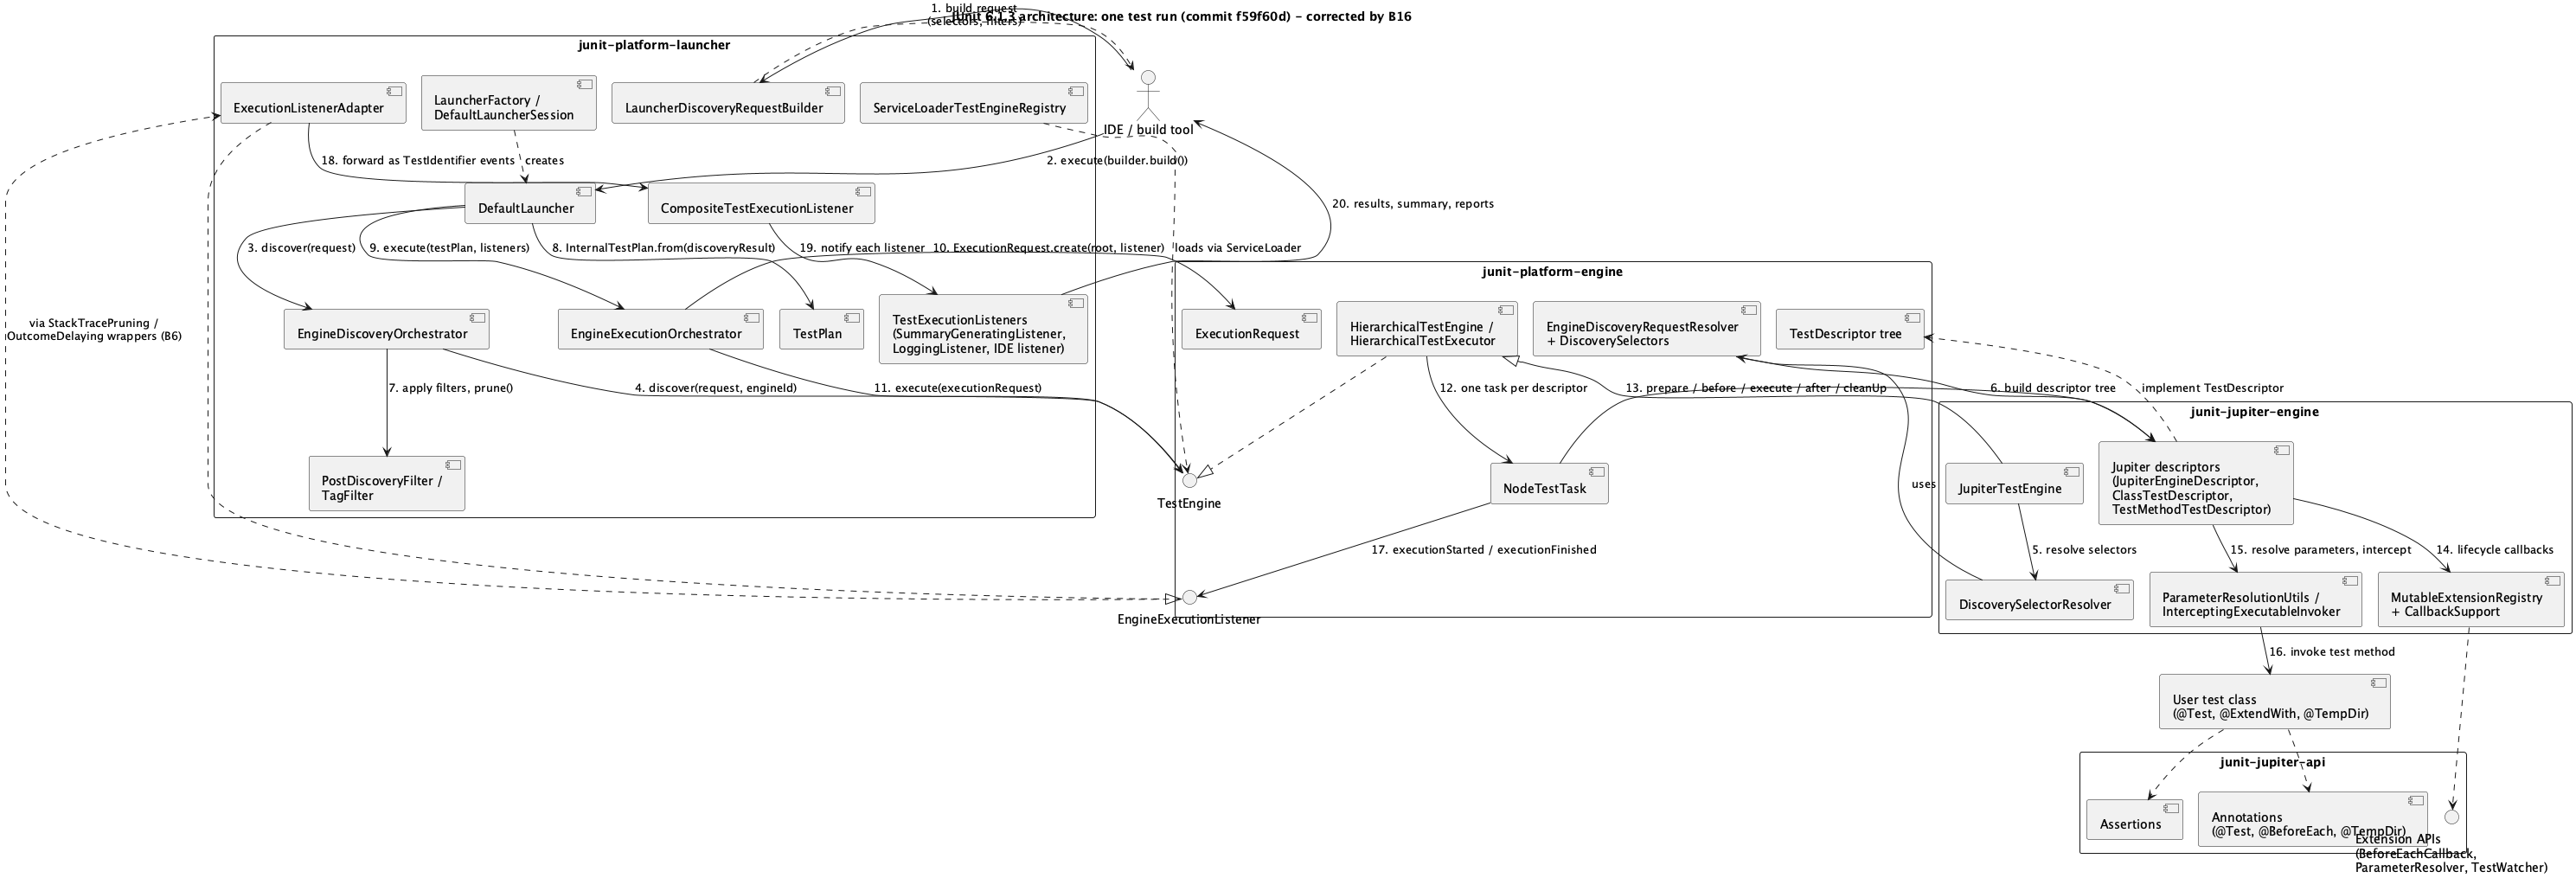
\includegraphics[width=\linewidth,height=0.48\textheight,keepaspectratio]{Part1/architecture/architecture.png}
\caption{Components and numbered flow of one test run (\protect\path{Part1/architecture/architecture.puml}; the LLM's original version and the two corrections are in the same folder).}\label{fig:arch}
\end{figure}

\entry{Run instructions}\path{README.md} (team folder). The JUnit fork is built and tested from its root with \path{./gradlew --no-configuration-cache --no-build-cache :platform-tests:test --rerun --tests "org.junit.platform.launcher.*"} (and \path{:jupiter-tests:test}). Actual results at the baseline: 382/382 launcher tests, 2452 platform tests and 3381 Jupiter tests passed (0 failures; 6 and 165 skipped by design). Logs: \path{Part2/changes/baseline_launcher_tests.log}, \path{Part2/changes/baseline_all_platform_tests.log}, \path{Part2/changes/Change2/before_all_jupiter_tests.log}.

\section{Part 1 Pattern discovery}
\entry{Method}For each area I first asked the LLM (Claude Opus 5.5) to list the files and explain the runtime flow, checked that answer in the source, and only then asked for pattern candidates with roles, files and line numbers (12 prompts, \path{Part1/llm/}). Every claimed line was checked automatically (\path{Part1/evidence/check_lines.py}) and every role by reading the code; 102 claims are recorded in \path{Part1/evidence/verification.csv}. Two counting rules were fixed before counting: (1) \emph{Composite rule}: a class is a Composite only if it combines children of its own interface \emph{and} merges their answers into one result; (2) two views of the same classes (A2/A3, B1/B2) are counted as separate instances with an overlap note, and a class found in two areas is counted once (B6--B8 are marked ``also Area C''). Line ranges in \path{data/patterns.csv} are computed from the source by \path{data/build_part1_csv.py}.

\subsection{Totals at the baseline}
\entry{Confirmed pattern types}10 (Strategy, Adapter, Observer, Decorator, Template Method, Composite, Command, Null Object, Chain of Responsibility, Factory Method)\par
\entry{Confirmed pattern instances}35\par
\entry{Concrete participant classes}76\par
\entry{Unique participant symbols}152 (177 role mappings; symbols shared by two instances counted once)\par
\entry{Rejected and uncertain candidates}25 rejected and 8 uncertain, observed in the same four modules at commit \texttt{f59f60d} (Table~\ref{tab:rejected}).

\subsection{Pattern inventory}
\begin{longtable}{@{}p{0.17\linewidth}p{0.57\linewidth}p{0.09\linewidth}p{0.11\linewidth}@{}}\toprule
Pattern type & Instance names & Instances & Concrete classes\\\midrule\endhead
Strategy & A3 Post-Discovery Filter Policies; B3 Test Executor Services; B4 Parallelism Configuration Strategy; C3 Listener Notification Order; C4 Pluggable Log Sink; D1 Temp Directory Creation; D2 Temp Directory Deletion; D3 Parameter Resolution; D4 Conditional Execution; D5 Store Close Action & 10 & 21\\
Adapter & A7 Orderer Descriptor Wrappers; B7 Engine-to-Launcher Listener Adapter; C5 Test Reporter Adapter; D6 Extension Store Adapter; D7 Lifecycle Method Adapters & 5 & 5\\
Observer & A6 Discovery Event Notification; B8 Execution Event Notification; C1 Test Execution Listeners; C2 Launcher Session Notification; D8 Test Outcome Watchers & 5 & 11\\
Decorator & B5 Intercepting Launcher Wrappers; B6 Engine Listener Wrappers; C6 Captured Output Stream; D10 Timeout Invocation Wrappers & 4 & 9\\
Template Method & A4 Jupiter Descriptor Skeletons; A5 Child Ordering Skeleton; B1 Hierarchical Engine Execution Skeleton & 3 & 6\\
Command & B9 Node Execution Tasks; D11 Packaged Reflective Calls & 2 & 3\\
Composite & A1 Test Descriptor Tree; A2 Composed Discovery Filter & 2 & 15\\
Null Object & B10 No-op Node; C7 No-op Listeners & 2 & 3\\
Chain of Responsibility & D9 Invocation Interceptor Chain & 1 & 1\\
Factory Method & B2 Engine Collaborator Factory Methods & 1 & 2\\
\midrule\textbf{Total} & 10 pattern types & \textbf{35} & \textbf{76}\\
\bottomrule\end{longtable}

\subsection{One record for each pattern instance}
Each record gives the pattern, the purpose (as evidence) and every participant with its file and line range. Paths are shortened to module/.../file; the full paths are in \path{data/patterns.csv}. All instances are JUnit framework code. Each record names its diagram; PlantUML sources and PNGs for all 35 instances are in \path{Part1/uml/}.

\subsubsection*{Area A: discovery and test descriptors}
\paragraph{A1 Test Descriptor Tree} \textbf{Pattern:} Composite (Structural, GoF). \textbf{Origin:} JUnit framework code (not student-added). \textbf{Concrete participant classes:} 12.\par
\begin{longtable}{@{}p{0.19\linewidth}p{0.41\linewidth}p{0.33\linewidth}@{}}\toprule
Role & Class / interface / function & File and lines\\\midrule\endhead
Component & \texttt{org.\allowbreak{}junit.\allowbreak{}platform.\allowbreak{}engine.\allowbreak{}Test\allowbreak{}Descriptor} & \path{junit-platform-engine/.../TestDescriptor.java:37-427}\\
Composite (base) & \texttt{org.\allowbreak{}junit.\allowbreak{}platform.\allowbreak{}engine.\allowbreak{}support.\allowbreak{}descriptor.\allowbreak{}Abstract\allowbreak{}Test\allowbreak{}Descriptor} & \path{junit-platform-engine/.../AbstractTestDescriptor.java:42-248}\\
Composite & \texttt{org.\allowbreak{}junit.\allowbreak{}platform.\allowbreak{}engine.\allowbreak{}support.\allowbreak{}descriptor.\allowbreak{}Engine\allowbreak{}Descriptor} & \path{junit-platform-engine/.../EngineDescriptor.java:25-53}\\
Composite & \texttt{org.\allowbreak{}junit.\allowbreak{}jupiter.\allowbreak{}engine.\allowbreak{}descriptor.\allowbreak{}Jupiter\allowbreak{}Engine\allowbreak{}Descriptor} & \path{junit-jupiter-engine/.../JupiterEngineDescriptor.java:30-70}\\
Composite & \texttt{org.\allowbreak{}junit.\allowbreak{}jupiter.\allowbreak{}engine.\allowbreak{}descriptor.\allowbreak{}Class\allowbreak{}Test\allowbreak{}Descriptor} & \path{junit-jupiter-engine/.../ClassTestDescriptor.java:47-106}\\
Composite & \texttt{org.\allowbreak{}junit.\allowbreak{}jupiter.\allowbreak{}engine.\allowbreak{}descriptor.\allowbreak{}Nested\allowbreak{}Class\allowbreak{}Test\allowbreak{}Descriptor} & \path{junit-jupiter-engine/.../NestedClassTestDescriptor.java:49-121}\\
Composite & \texttt{org.\allowbreak{}junit.\allowbreak{}jupiter.\allowbreak{}engine.\allowbreak{}descriptor.\allowbreak{}Class\allowbreak{}Template\allowbreak{}Test\allowbreak{}Descriptor} & \path{junit-jupiter-engine/.../ClassTemplateTestDescriptor.java:51-277}\\
Composite & \texttt{org.\allowbreak{}junit.\allowbreak{}jupiter.\allowbreak{}engine.\allowbreak{}descriptor.\allowbreak{}Class\allowbreak{}Template\allowbreak{}Invocation\allowbreak{}Test\allowbreak{}Descriptor} & \path{junit-jupiter-engine/.../ClassTemplateInvocationTestDescriptor.java:48-202}\\
Composite & \texttt{org.\allowbreak{}junit.\allowbreak{}jupiter.\allowbreak{}engine.\allowbreak{}descriptor.\allowbreak{}Test\allowbreak{}Template\allowbreak{}Test\allowbreak{}Descriptor} & \path{junit-jupiter-engine/.../TestTemplateTestDescriptor.java:41-167}\\
Composite & \texttt{org.\allowbreak{}junit.\allowbreak{}jupiter.\allowbreak{}engine.\allowbreak{}descriptor.\allowbreak{}Test\allowbreak{}Factory\allowbreak{}Test\allowbreak{}Descriptor} & \path{junit-jupiter-engine/.../TestFactoryTestDescriptor.java:56-223}\\
Composite & \texttt{org.\allowbreak{}junit.\allowbreak{}jupiter.\allowbreak{}engine.\allowbreak{}descriptor.\allowbreak{}Dynamic\allowbreak{}Container\allowbreak{}Test\allowbreak{}Descriptor} & \path{junit-jupiter-engine/.../DynamicContainerTestDescriptor.java:34-88}\\
Leaf & \texttt{org.\allowbreak{}junit.\allowbreak{}jupiter.\allowbreak{}engine.\allowbreak{}descriptor.\allowbreak{}Test\allowbreak{}Method\allowbreak{}Test\allowbreak{}Descriptor} & \path{junit-jupiter-engine/.../TestMethodTestDescriptor.java:71-293}\\
Leaf & \texttt{org.\allowbreak{}junit.\allowbreak{}jupiter.\allowbreak{}engine.\allowbreak{}descriptor.\allowbreak{}Test\allowbreak{}Template\allowbreak{}Invocation\allowbreak{}Test\allowbreak{}Descriptor} & \path{junit-jupiter-engine/.../TestTemplateInvocationTestDescriptor.java:42-104}\\
Leaf & \texttt{org.\allowbreak{}junit.\allowbreak{}jupiter.\allowbreak{}engine.\allowbreak{}descriptor.\allowbreak{}Dynamic\allowbreak{}Test\allowbreak{}Test\allowbreak{}Descriptor} & \path{junit-jupiter-engine/.../DynamicTestTestDescriptor.java:37-100}\\
Client & \texttt{org.\allowbreak{}junit.\allowbreak{}platform.\allowbreak{}launcher.\allowbreak{}core.\allowbreak{}Engine\allowbreak{}Discovery\allowbreak{}Orchestrator\#\allowbreak{}apply\allowbreak{}Post\allowbreak{}Discovery\allowbreak{}Filters} & \path{junit-platform-launcher/.../EngineDiscoveryOrchestrator.java:225-238}\\
Client & \texttt{org.\allowbreak{}junit.\allowbreak{}platform.\allowbreak{}engine.\allowbreak{}support.\allowbreak{}hierarchical.\allowbreak{}Node\allowbreak{}Test\allowbreak{}Task\#\allowbreak{}execute\allowbreak{}Recursively} & \path{junit-platform-engine/.../NodeTestTask.java:157-189}\\
\bottomrule\end{longtable}
\textbf{Evidence:} Engines build one tree of TestDescriptor nodes (engine \textgreater{} class \textgreater{} nested class \textgreater{} method \textgreater{} dynamic test); the launcher filters, prunes, visits and executes it without knowing node kinds. Evidence: TestDescriptor.accept visits itself then calls child.accept(visitor); AbstractTestDescriptor holds the children set and findByUniqueId recurses; NodeTestTask creates one child task per child. Transparent variant: leaf vs container is decided by getType().\par
\textbf{Key code:} \texttt{this.\allowbreak{}get\allowbreak{}Children().\allowbreak{}for\allowbreak{}Each(child -\textgreater{} child.\allowbreak{}accept(visitor));} (TestDescriptor.java:348)\par
\textbf{Diagram:} \path{Part1/uml/png/A1.png} (source in \path{Part1/uml/}). \textbf{Verification:} confirmed (reviewer: Gautham Mohanraj); claims and line numbers checked in \path{Part1/evidence/verification.csv}, decisions in \path{Part1/notes.md}.\par
\paragraph{A2 Composed Discovery Filter} \textbf{Pattern:} Composite (Structural, GoF). \textbf{Origin:} JUnit framework code (not student-added). \textbf{Concrete participant classes:} 3.\par
\begin{longtable}{@{}p{0.19\linewidth}p{0.41\linewidth}p{0.33\linewidth}@{}}\toprule
Role & Class / interface / function & File and lines\\\midrule\endhead
Component & \texttt{org.\allowbreak{}junit.\allowbreak{}platform.\allowbreak{}engine.\allowbreak{}Filter} & \path{junit-platform-engine/.../Filter.java:41-119}\\
Composite & \texttt{org.\allowbreak{}junit.\allowbreak{}platform.\allowbreak{}engine.\allowbreak{}Composite\allowbreak{}Filter} & \path{junit-platform-engine/.../CompositeFilter.java:29-89}\\
Leaf & \texttt{org.\allowbreak{}junit.\allowbreak{}platform.\allowbreak{}launcher.\allowbreak{}Include\allowbreak{}Method\allowbreak{}Filter} & \path{junit-platform-launcher/.../IncludeMethodFilter.java:31-58}\\
Leaf & \texttt{org.\allowbreak{}junit.\allowbreak{}platform.\allowbreak{}launcher.\allowbreak{}Exclude\allowbreak{}Method\allowbreak{}Filter} & \path{junit-platform-launcher/.../ExcludeMethodFilter.java:31-58}\\
Leaf (lambda factory) & \texttt{org.\allowbreak{}junit.\allowbreak{}platform.\allowbreak{}launcher.\allowbreak{}Tag\allowbreak{}Filter} & \path{junit-platform-launcher/.../TagFilter.java:48-184}\\
Client & \texttt{org.\allowbreak{}junit.\allowbreak{}platform.\allowbreak{}launcher.\allowbreak{}core.\allowbreak{}Engine\allowbreak{}Discovery\allowbreak{}Orchestrator\#\allowbreak{}apply\allowbreak{}Post\allowbreak{}Discovery\allowbreak{}Filters} & \path{junit-platform-launcher/.../EngineDiscoveryOrchestrator.java:225-238}\\
\bottomrule\end{longtable}
\textbf{Evidence:} All post-discovery filters are merged into one Filter by Filter.composeFilters; CompositeFilter implements Filter, holds a list of Filters and combines their FilterResults into one answer (first exclusion wins). Overlaps A3 (same leaf classes seen as strategies).\par
\textbf{Key code:} \texttt{.\allowbreak{}map(filter -\textgreater{} filter.\allowbreak{}apply(element))} (CompositeFilter.java:62)\par
\textbf{Diagram:} \path{Part1/uml/png/A2.png} (source in \path{Part1/uml/}). \textbf{Verification:} confirmed (reviewer: Gautham Mohanraj); claims and line numbers checked in \path{Part1/evidence/verification.csv}, decisions in \path{Part1/notes.md}.\par
\paragraph{A3 Post-Discovery Filter Policies} \textbf{Pattern:} Strategy (Behavioral, GoF). \textbf{Origin:} JUnit framework code (not student-added). \textbf{Concrete participant classes:} 3.\par
\begin{longtable}{@{}p{0.19\linewidth}p{0.41\linewidth}p{0.33\linewidth}@{}}\toprule
Role & Class / interface / function & File and lines\\\midrule\endhead
Strategy & \texttt{org.\allowbreak{}junit.\allowbreak{}platform.\allowbreak{}launcher.\allowbreak{}Post\allowbreak{}Discovery\allowbreak{}Filter} & \path{junit-platform-launcher/.../PostDiscoveryFilter.java:35-36}\\
ConcreteStrategy & \texttt{org.\allowbreak{}junit.\allowbreak{}platform.\allowbreak{}launcher.\allowbreak{}Include\allowbreak{}Method\allowbreak{}Filter} & \path{junit-platform-launcher/.../IncludeMethodFilter.java:31-58}\\
ConcreteStrategy & \texttt{org.\allowbreak{}junit.\allowbreak{}platform.\allowbreak{}launcher.\allowbreak{}Exclude\allowbreak{}Method\allowbreak{}Filter} & \path{junit-platform-launcher/.../ExcludeMethodFilter.java:31-58}\\
ConcreteStrategy (lambdas) & \texttt{org.\allowbreak{}junit.\allowbreak{}platform.\allowbreak{}launcher.\allowbreak{}Tag\allowbreak{}Filter} & \path{junit-platform-launcher/.../TagFilter.java:48-184}\\
Context & \texttt{org.\allowbreak{}junit.\allowbreak{}platform.\allowbreak{}launcher.\allowbreak{}core.\allowbreak{}Engine\allowbreak{}Discovery\allowbreak{}Orchestrator\#\allowbreak{}apply\allowbreak{}Post\allowbreak{}Discovery\allowbreak{}Filters} & \path{junit-platform-launcher/.../EngineDiscoveryOrchestrator.java:225-238}\\
\bottomrule\end{longtable}
\textbf{Evidence:} Selection rules (tag expressions, method-name patterns, custom filters) are interchangeable algorithms behind PostDiscoveryFilter; EngineDiscoveryOrchestrator only calls apply(). Overlaps A2.\par
\textbf{Key code:} \texttt{Filter\allowbreak{}Result filter\allowbreak{}Result = post\allowbreak{}Discovery\allowbreak{}Filter.\allowbreak{}apply(descriptor);} (EngineDiscoveryOrchestrator.java:230)\par
\textbf{Diagram:} \path{Part1/uml/png/A3.png} (source in \path{Part1/uml/}). \textbf{Verification:} confirmed (reviewer: Gautham Mohanraj); claims and line numbers checked in \path{Part1/evidence/verification.csv}, decisions in \path{Part1/notes.md}.\par
\paragraph{A4 Jupiter Descriptor Skeletons} \textbf{Pattern:} Template Method (Behavioral, GoF). \textbf{Origin:} JUnit framework code (not student-added). \textbf{Concrete participant classes:} 3.\par
\begin{longtable}{@{}p{0.19\linewidth}p{0.41\linewidth}p{0.33\linewidth}@{}}\toprule
Role & Class / interface / function & File and lines\\\midrule\endhead
AbstractClass & \texttt{org.\allowbreak{}junit.\allowbreak{}jupiter.\allowbreak{}engine.\allowbreak{}descriptor.\allowbreak{}Jupiter\allowbreak{}Test\allowbreak{}Descriptor} & \path{junit-jupiter-engine/.../JupiterTestDescriptor.java:64-283}\\
TemplateMethod & \texttt{org.\allowbreak{}junit.\allowbreak{}jupiter.\allowbreak{}engine.\allowbreak{}descriptor.\allowbreak{}Jupiter\allowbreak{}Test\allowbreak{}Descriptor\#\allowbreak{}get\allowbreak{}Execution\allowbreak{}Mode} & \path{junit-jupiter-engine/.../JupiterTestDescriptor.java:163-167}\\
TemplateMethod & \texttt{org.\allowbreak{}junit.\allowbreak{}jupiter.\allowbreak{}engine.\allowbreak{}descriptor.\allowbreak{}Jupiter\allowbreak{}Test\allowbreak{}Descriptor\#\allowbreak{}get\allowbreak{}Legacy\allowbreak{}Reporting\allowbreak{}Name} & \path{junit-jupiter-engine/.../JupiterTestDescriptor.java:85-88}\\
TemplateMethod & \texttt{org.\allowbreak{}junit.\allowbreak{}jupiter.\allowbreak{}engine.\allowbreak{}descriptor.\allowbreak{}Jupiter\allowbreak{}Test\allowbreak{}Descriptor\#\allowbreak{}copy\allowbreak{}Including\allowbreak{}Descendants} & \path{junit-jupiter-engine/.../JupiterTestDescriptor.java:256-263}\\
PrimitiveOperation & \texttt{org.\allowbreak{}junit.\allowbreak{}jupiter.\allowbreak{}engine.\allowbreak{}descriptor.\allowbreak{}Jupiter\allowbreak{}Test\allowbreak{}Descriptor\#\allowbreak{}with\allowbreak{}Unique\allowbreak{}Id} & \path{junit-jupiter-engine/.../JupiterTestDescriptor.java:268-268}\\
ConcreteClass (hook) & \texttt{org.\allowbreak{}junit.\allowbreak{}jupiter.\allowbreak{}engine.\allowbreak{}descriptor.\allowbreak{}Class\allowbreak{}Based\allowbreak{}Test\allowbreak{}Descriptor\#\allowbreak{}get\allowbreak{}Explicit\allowbreak{}Execution\allowbreak{}Mode} & \path{junit-jupiter-engine/.../ClassBasedTestDescriptor.java:167-169}\\
ConcreteClass (hook) & \texttt{org.\allowbreak{}junit.\allowbreak{}jupiter.\allowbreak{}engine.\allowbreak{}descriptor.\allowbreak{}Method\allowbreak{}Based\allowbreak{}Test\allowbreak{}Descriptor\#\allowbreak{}get\allowbreak{}Explicit\allowbreak{}Execution\allowbreak{}Mode} & \path{junit-jupiter-engine/.../MethodBasedTestDescriptor.java:147-149}\\
ConcreteClass (primitive) & \texttt{org.\allowbreak{}junit.\allowbreak{}jupiter.\allowbreak{}engine.\allowbreak{}descriptor.\allowbreak{}Class\allowbreak{}Test\allowbreak{}Descriptor\#\allowbreak{}with\allowbreak{}Unique\allowbreak{}Id} & \path{junit-jupiter-engine/.../ClassTestDescriptor.java:63-66}\\
\bottomrule\end{longtable}
\textbf{Evidence:} JupiterTestDescriptor fixes algorithms in final methods (getExecutionMode, getLegacyReportingName) and in copyIncludingDescendants, which calls the abstract primitive withUniqueId; subclasses override the hooks (getExplicitExecutionMode, getLegacyReportingBaseName, withUniqueId).\par
\textbf{Key code:} \texttt{public final Execution\allowbreak{}Mode get\allowbreak{}Execution\allowbreak{}Mode() \{} (JupiterTestDescriptor.java:163; see JupiterTestDescriptor.java:163, 268)\par
\textbf{Diagram:} \path{Part1/uml/png/A4.png} (source in \path{Part1/uml/}). \textbf{Verification:} confirmed (reviewer: Gautham Mohanraj); claims and line numbers checked in \path{Part1/evidence/verification.csv}, decisions in \path{Part1/notes.md}.\par
\paragraph{A5 Child Ordering Skeleton} \textbf{Pattern:} Template Method (Behavioral, GoF). \textbf{Origin:} JUnit framework code (not student-added). \textbf{Concrete participant classes:} 2.\par
\begin{longtable}{@{}p{0.19\linewidth}p{0.41\linewidth}p{0.33\linewidth}@{}}\toprule
Role & Class / interface / function & File and lines\\\midrule\endhead
AbstractClass & \texttt{org.\allowbreak{}junit.\allowbreak{}jupiter.\allowbreak{}engine.\allowbreak{}discovery.\allowbreak{}Abstract\allowbreak{}Ordering\allowbreak{}Visitor} & \path{junit-jupiter-engine/.../AbstractOrderingVisitor.java:39-222}\\
TemplateMethod & \texttt{org.\allowbreak{}junit.\allowbreak{}jupiter.\allowbreak{}engine.\allowbreak{}discovery.\allowbreak{}Abstract\allowbreak{}Ordering\allowbreak{}Visitor\#\allowbreak{}order\allowbreak{}Children\allowbreak{}Test\allowbreak{}Descriptors} & \path{junit-jupiter-engine/.../AbstractOrderingVisitor.java:72-119}\\
PrimitiveOperation & \texttt{org.\allowbreak{}junit.\allowbreak{}jupiter.\allowbreak{}engine.\allowbreak{}discovery.\allowbreak{}Abstract\allowbreak{}Ordering\allowbreak{}Visitor\#\allowbreak{}should\allowbreak{}Non\allowbreak{}Matching\allowbreak{}Descriptors\allowbreak{}Come\allowbreak{}Before\allowbreak{}Ordered\allowbreak{}Ones} & \path{junit-jupiter-engine/.../AbstractOrderingVisitor.java:126-126}\\
ConcreteClass & \texttt{org.\allowbreak{}junit.\allowbreak{}jupiter.\allowbreak{}engine.\allowbreak{}discovery.\allowbreak{}Class\allowbreak{}Ordering\allowbreak{}Visitor} & \path{junit-jupiter-engine/.../ClassOrderingVisitor.java:38-165}\\
ConcreteClass & \texttt{org.\allowbreak{}junit.\allowbreak{}jupiter.\allowbreak{}engine.\allowbreak{}discovery.\allowbreak{}Method\allowbreak{}Ordering\allowbreak{}Visitor} & \path{junit-jupiter-engine/.../MethodOrderingVisitor.java:41-174}\\
\bottomrule\end{longtable}
\textbf{Evidence:} AbstractOrderingVisitor.orderChildrenTestDescriptors runs a fixed ordering algorithm (select, wrap, sort, unwrap, merge) and asks the abstract hook shouldNonMatchingDescriptorsComeBeforeOrderedOnes, which ClassOrderingVisitor and MethodOrderingVisitor answer differently.\par
\textbf{Key code:} \texttt{if (should\allowbreak{}Non\allowbreak{}Matching\allowbreak{}Descriptors\allowbreak{}Come\allowbreak{}Before\allowbreak{}Ordered\allowbreak{}Ones()) \{} (AbstractOrderingVisitor.java:110; see AbstractOrderingVisitor.java:110, 126)\par
\textbf{Diagram:} \path{Part1/uml/png/A5.png} (source in \path{Part1/uml/}). \textbf{Verification:} confirmed (reviewer: Gautham Mohanraj); claims and line numbers checked in \path{Part1/evidence/verification.csv}, decisions in \path{Part1/notes.md}.\par
\paragraph{A6 Discovery Event Notification} \textbf{Pattern:} Observer (Behavioral, GoF). \textbf{Origin:} JUnit framework code (not student-added). \textbf{Concrete participant classes:} 2.\par
\begin{longtable}{@{}p{0.19\linewidth}p{0.41\linewidth}p{0.33\linewidth}@{}}\toprule
Role & Class / interface / function & File and lines\\\midrule\endhead
Observer & \texttt{org.\allowbreak{}junit.\allowbreak{}platform.\allowbreak{}launcher.\allowbreak{}Launcher\allowbreak{}Discovery\allowbreak{}Listener} & \path{junit-platform-launcher/.../LauncherDiscoveryListener.java:42-91}\\
Observer (base) & \texttt{org.\allowbreak{}junit.\allowbreak{}platform.\allowbreak{}engine.\allowbreak{}Engine\allowbreak{}Discovery\allowbreak{}Listener} & \path{junit-platform-engine/.../EngineDiscoveryListener.java:31-67}\\
ConcreteObserver & \texttt{org.\allowbreak{}junit.\allowbreak{}platform.\allowbreak{}launcher.\allowbreak{}core.\allowbreak{}Discovery\allowbreak{}Issue\allowbreak{}Collector} & \path{junit-platform-launcher/.../DiscoveryIssueCollector.java:25-65}\\
ConcreteObserver & \texttt{org.\allowbreak{}junit.\allowbreak{}platform.\allowbreak{}launcher.\allowbreak{}core.\allowbreak{}Discovery\allowbreak{}Issue\allowbreak{}Reporting\allowbreak{}Discovery\allowbreak{}Listener} & \path{junit-platform-launcher/.../DiscoveryIssueReportingDiscoveryListener.java:49-131}\\
Subject (attach) & \texttt{org.\allowbreak{}junit.\allowbreak{}platform.\allowbreak{}launcher.\allowbreak{}core.\allowbreak{}Default\allowbreak{}Launcher\#\allowbreak{}register\allowbreak{}Launcher\allowbreak{}Discovery\allowbreak{}Listeners} & \path{junit-platform-launcher/.../DefaultLauncher.java:73-77}\\
Subject (notify) & \texttt{org.\allowbreak{}junit.\allowbreak{}platform.\allowbreak{}launcher.\allowbreak{}core.\allowbreak{}Engine\allowbreak{}Discovery\allowbreak{}Orchestrator\#\allowbreak{}discover\allowbreak{}Engine\allowbreak{}Root} & \path{junit-platform-launcher/.../EngineDiscoveryOrchestrator.java:189-214}\\
Subject (notify, in engine) & \texttt{org.\allowbreak{}junit.\allowbreak{}platform.\allowbreak{}engine.\allowbreak{}support.\allowbreak{}discovery.\allowbreak{}Engine\allowbreak{}Discovery\allowbreak{}Request\allowbreak{}Resolution} & \path{junit-platform-engine/.../EngineDiscoveryRequestResolution.java:60-263}\\
Multicaster & \texttt{org.\allowbreak{}junit.\allowbreak{}platform.\allowbreak{}launcher.\allowbreak{}listeners.\allowbreak{}discovery.\allowbreak{}Composite\allowbreak{}Launcher\allowbreak{}Discovery\allowbreak{}Listener} & \path{junit-platform-launcher/.../CompositeLauncherDiscoveryListener.java:29-67}\\
\bottomrule\end{longtable}
\textbf{Evidence:} Discovery progress (launcher/engine discovery started and finished, selector processed, issues) is pushed to registered LauncherDiscoveryListeners that the orchestrator only knows by interface.\par
\textbf{Key code:} \texttt{listener.\allowbreak{}engine\allowbreak{}Discovery\allowbreak{}Started(unique\allowbreak{}Engine\allowbreak{}Id);} (EngineDiscoveryOrchestrator.java:194; see EngineDiscoveryOrchestrator.java:194-197)\par
\textbf{Diagram:} \path{Part1/uml/png/A6.png} (source in \path{Part1/uml/}). \textbf{Verification:} confirmed (reviewer: Gautham Mohanraj); claims and line numbers checked in \path{Part1/evidence/verification.csv}, decisions in \path{Part1/notes.md}.\par
\paragraph{A7 Orderer Descriptor Wrappers} \textbf{Pattern:} Adapter (Structural, GoF). \textbf{Origin:} JUnit framework code (not student-added). \textbf{Concrete participant classes:} 2.\par
\begin{longtable}{@{}p{0.19\linewidth}p{0.41\linewidth}p{0.33\linewidth}@{}}\toprule
Role & Class / interface / function & File and lines\\\midrule\endhead
Target & \texttt{org.\allowbreak{}junit.\allowbreak{}jupiter.\allowbreak{}api.\allowbreak{}Class\allowbreak{}Descriptor} & \path{junit-jupiter-api/.../ClassDescriptor.java:28-87}\\
Target & \texttt{org.\allowbreak{}junit.\allowbreak{}jupiter.\allowbreak{}api.\allowbreak{}Method\allowbreak{}Descriptor} & \path{junit-jupiter-api/.../MethodDescriptor.java:29-90}\\
Adapter (base) & \texttt{org.\allowbreak{}junit.\allowbreak{}jupiter.\allowbreak{}engine.\allowbreak{}discovery.\allowbreak{}Abstract\allowbreak{}Annotated\allowbreak{}Descriptor\allowbreak{}Wrapper} & \path{junit-jupiter-engine/.../AbstractAnnotatedDescriptorWrapper.java:28-65}\\
Adapter & \texttt{org.\allowbreak{}junit.\allowbreak{}jupiter.\allowbreak{}engine.\allowbreak{}discovery.\allowbreak{}Default\allowbreak{}Class\allowbreak{}Descriptor} & \path{junit-jupiter-engine/.../DefaultClassDescriptor.java:23-39}\\
Adapter & \texttt{org.\allowbreak{}junit.\allowbreak{}jupiter.\allowbreak{}engine.\allowbreak{}discovery.\allowbreak{}Default\allowbreak{}Method\allowbreak{}Descriptor} & \path{junit-jupiter-engine/.../DefaultMethodDescriptor.java:25-41}\\
Adaptee & \texttt{org.\allowbreak{}junit.\allowbreak{}jupiter.\allowbreak{}engine.\allowbreak{}descriptor.\allowbreak{}Class\allowbreak{}Based\allowbreak{}Test\allowbreak{}Descriptor} & \path{junit-jupiter-engine/.../ClassBasedTestDescriptor.java:89-601}\\
Adaptee & \texttt{org.\allowbreak{}junit.\allowbreak{}jupiter.\allowbreak{}engine.\allowbreak{}descriptor.\allowbreak{}Method\allowbreak{}Based\allowbreak{}Test\allowbreak{}Descriptor} & \path{junit-jupiter-engine/.../MethodBasedTestDescriptor.java:56-217}\\
Client & \texttt{org.\allowbreak{}junit.\allowbreak{}jupiter.\allowbreak{}engine.\allowbreak{}discovery.\allowbreak{}Class\allowbreak{}Ordering\allowbreak{}Visitor} & \path{junit-jupiter-engine/.../ClassOrderingVisitor.java:38-165}\\
\bottomrule\end{longtable}
\textbf{Evidence:} User ClassOrderer/MethodOrderer code expects the public ClassDescriptor/MethodDescriptor API; the wrappers expose internal descriptors through it so internal classes never leak to user code.\par
\textbf{Key code:} \texttt{class Default\allowbreak{}Class\allowbreak{}Descriptor extends Abstract\allowbreak{}Annotated\allowbreak{}Descriptor\allowbreak{}Wrapper\textless{}Class\textless{}?\textgreater{}\textgreater{} implements Class\allowbreak{}Descriptor \{} (DefaultClassDescriptor.java:23; see DefaultClassDescriptor.java:23-26)\par
\textbf{Diagram:} \path{Part1/uml/png/A7.png} (source in \path{Part1/uml/}). \textbf{Verification:} confirmed (reviewer: Gautham Mohanraj); claims and line numbers checked in \path{Part1/evidence/verification.csv}, decisions in \path{Part1/notes.md}.\par
\subsubsection*{Area B: engines and execution lifecycle}
\paragraph{B1 Hierarchical Engine Execution Skeleton} \textbf{Pattern:} Template Method (Behavioral, GoF). \textbf{Origin:} JUnit framework code (not student-added). \textbf{Concrete participant classes:} 1.\par
\begin{longtable}{@{}p{0.19\linewidth}p{0.41\linewidth}p{0.33\linewidth}@{}}\toprule
Role & Class / interface / function & File and lines\\\midrule\endhead
AbstractClass & \texttt{org.\allowbreak{}junit.\allowbreak{}platform.\allowbreak{}engine.\allowbreak{}support.\allowbreak{}hierarchical.\allowbreak{}Hierarchical\allowbreak{}Test\allowbreak{}Engine} & \path{junit-platform-engine/.../HierarchicalTestEngine.java:31-119}\\
TemplateMethod & \texttt{org.\allowbreak{}junit.\allowbreak{}platform.\allowbreak{}engine.\allowbreak{}support.\allowbreak{}hierarchical.\allowbreak{}Hierarchical\allowbreak{}Test\allowbreak{}Engine\#\allowbreak{}execute} & \path{junit-platform-engine/.../HierarchicalTestEngine.java:53-63}\\
PrimitiveOperation & \texttt{org.\allowbreak{}junit.\allowbreak{}platform.\allowbreak{}engine.\allowbreak{}support.\allowbreak{}hierarchical.\allowbreak{}Hierarchical\allowbreak{}Test\allowbreak{}Engine\#\allowbreak{}create\allowbreak{}Execution\allowbreak{}Context} & \path{junit-platform-engine/.../HierarchicalTestEngine.java:117-117}\\
ConcreteClass & \texttt{org.\allowbreak{}junit.\allowbreak{}jupiter.\allowbreak{}engine.\allowbreak{}Jupiter\allowbreak{}Test\allowbreak{}Engine} & \path{junit-jupiter-engine/.../JupiterTestEngine.java:44-108}\\
\bottomrule\end{longtable}
\textbf{Evidence:} final HierarchicalTestEngine.execute fixes the run order (executor service, context, collector factory, HierarchicalTestExecutor); JupiterTestEngine only supplies the steps. Overlaps B2.\par
\textbf{Key code:} \texttt{public final void execute(Execution\allowbreak{}Request request) \{} (HierarchicalTestEngine.java:53; see HierarchicalTestEngine.java:53-59, 117)\par
\textbf{Diagram:} \path{Part1/uml/png/B1.png} (source in \path{Part1/uml/}). \textbf{Verification:} confirmed (reviewer: Gautham Mohanraj); claims and line numbers checked in \path{Part1/evidence/verification.csv}, decisions in \path{Part1/notes.md}.\par
\paragraph{B2 Engine Collaborator Factory Methods} \textbf{Pattern:} Factory Method (Creational, GoF). \textbf{Origin:} JUnit framework code (not student-added). \textbf{Concrete participant classes:} 2.\par
\begin{longtable}{@{}p{0.19\linewidth}p{0.41\linewidth}p{0.33\linewidth}@{}}\toprule
Role & Class / interface / function & File and lines\\\midrule\endhead
Creator (factory method) & \texttt{org.\allowbreak{}junit.\allowbreak{}platform.\allowbreak{}engine.\allowbreak{}support.\allowbreak{}hierarchical.\allowbreak{}Hierarchical\allowbreak{}Test\allowbreak{}Engine\#\allowbreak{}create\allowbreak{}Executor\allowbreak{}Service} & \path{junit-platform-engine/.../HierarchicalTestEngine.java:83-85}\\
ConcreteCreator & \texttt{org.\allowbreak{}junit.\allowbreak{}jupiter.\allowbreak{}engine.\allowbreak{}Jupiter\allowbreak{}Test\allowbreak{}Engine\#\allowbreak{}create\allowbreak{}Executor\allowbreak{}Service} & \path{junit-jupiter-engine/.../JupiterTestEngine.java:80-87}\\
ConcreteCreator & \texttt{org.\allowbreak{}junit.\allowbreak{}jupiter.\allowbreak{}engine.\allowbreak{}Jupiter\allowbreak{}Test\allowbreak{}Engine\#\allowbreak{}create\allowbreak{}Execution\allowbreak{}Context} & \path{junit-jupiter-engine/.../JupiterTestEngine.java:90-93}\\
ConcreteCreator & \texttt{org.\allowbreak{}junit.\allowbreak{}jupiter.\allowbreak{}engine.\allowbreak{}Jupiter\allowbreak{}Test\allowbreak{}Engine\#\allowbreak{}create\allowbreak{}Throwable\allowbreak{}Collector\allowbreak{}Factory} & \path{junit-jupiter-engine/.../JupiterTestEngine.java:99-101}\\
ConcreteProduct & \texttt{org.\allowbreak{}junit.\allowbreak{}jupiter.\allowbreak{}engine.\allowbreak{}execution.\allowbreak{}Jupiter\allowbreak{}Engine\allowbreak{}Execution\allowbreak{}Context} & \path{junit-jupiter-engine/.../JupiterEngineExecutionContext.java:30-209}\\
\bottomrule\end{longtable}
\textbf{Evidence:} The template in B1 asks overridable create* methods which objects to use; JupiterTestEngine overrides them to choose a parallel/same-thread executor, its JupiterEngineExecutionContext and its throwable-collector factory. Overlaps B1.\par
\textbf{Key code:} \texttt{protected Hierarchical\allowbreak{}Test\allowbreak{}Executor\allowbreak{}Service create\allowbreak{}Executor\allowbreak{}Service(Execution\allowbreak{}Request request) \{} (JupiterTestEngine.java:80; see JupiterTestEngine.java:80-100)\par
\textbf{Diagram:} \path{Part1/uml/png/B2.png} (source in \path{Part1/uml/}). \textbf{Verification:} confirmed (reviewer: Gautham Mohanraj); claims and line numbers checked in \path{Part1/evidence/verification.csv}, decisions in \path{Part1/notes.md}.\par
\paragraph{B3 Test Executor Services} \textbf{Pattern:} Strategy (Behavioral, GoF). \textbf{Origin:} JUnit framework code (not student-added). \textbf{Concrete participant classes:} 3.\par
\begin{longtable}{@{}p{0.19\linewidth}p{0.41\linewidth}p{0.33\linewidth}@{}}\toprule
Role & Class / interface / function & File and lines\\\midrule\endhead
Strategy & \texttt{org.\allowbreak{}junit.\allowbreak{}platform.\allowbreak{}engine.\allowbreak{}support.\allowbreak{}hierarchical.\allowbreak{}Hierarchical\allowbreak{}Test\allowbreak{}Executor\allowbreak{}Service} & \path{junit-platform-engine/.../HierarchicalTestExecutorService.java:34-118}\\
ConcreteStrategy & \texttt{org.\allowbreak{}junit.\allowbreak{}platform.\allowbreak{}engine.\allowbreak{}support.\allowbreak{}hierarchical.\allowbreak{}Same\allowbreak{}Thread\allowbreak{}Hierarchical\allowbreak{}Test\allowbreak{}Executor\allowbreak{}Service} & \path{junit-platform-engine/.../SameThreadHierarchicalTestExecutorService.java:29-50}\\
ConcreteStrategy & \texttt{org.\allowbreak{}junit.\allowbreak{}platform.\allowbreak{}engine.\allowbreak{}support.\allowbreak{}hierarchical.\allowbreak{}Fork\allowbreak{}Join\allowbreak{}Pool\allowbreak{}Hierarchical\allowbreak{}Test\allowbreak{}Executor\allowbreak{}Service} & \path{junit-platform-engine/.../ForkJoinPoolHierarchicalTestExecutorService.java:51-331}\\
ConcreteStrategy & \texttt{org.\allowbreak{}junit.\allowbreak{}platform.\allowbreak{}engine.\allowbreak{}support.\allowbreak{}hierarchical.\allowbreak{}Worker\allowbreak{}Thread\allowbreak{}Pool\allowbreak{}Hierarchical\allowbreak{}Test\allowbreak{}Executor\allowbreak{}Service} & \path{junit-platform-engine/.../WorkerThreadPoolHierarchicalTestExecutorService.java:70-901}\\
Context & \texttt{org.\allowbreak{}junit.\allowbreak{}platform.\allowbreak{}engine.\allowbreak{}support.\allowbreak{}hierarchical.\allowbreak{}Hierarchical\allowbreak{}Test\allowbreak{}Executor} & \path{junit-platform-engine/.../HierarchicalTestExecutor.java:36-71}\\
Context & \texttt{org.\allowbreak{}junit.\allowbreak{}platform.\allowbreak{}engine.\allowbreak{}support.\allowbreak{}hierarchical.\allowbreak{}Node\allowbreak{}Test\allowbreak{}Task\#\allowbreak{}execute\allowbreak{}Recursively} & \path{junit-platform-engine/.../NodeTestTask.java:157-189}\\
\bottomrule\end{longtable}
\textbf{Evidence:} Sequential vs parallel scheduling is swappable behind HierarchicalTestExecutorService; NodeTestTask and HierarchicalTestExecutor only call submit/invokeAll.\par
\textbf{Key code:} \texttt{task\allowbreak{}Context.\allowbreak{}executor\allowbreak{}Service().\allowbreak{}invoke\allowbreak{}All(children);} (NodeTestTask.java:180)\par
\textbf{Diagram:} \path{Part1/uml/png/B3.png} (source in \path{Part1/uml/}). \textbf{Verification:} confirmed (reviewer: Gautham Mohanraj); claims and line numbers checked in \path{Part1/evidence/verification.csv}, decisions in \path{Part1/notes.md}.\par
\paragraph{B4 Parallelism Configuration Strategy} \textbf{Pattern:} Strategy (Behavioral, GoF). \textbf{Origin:} JUnit framework code (not student-added). \textbf{Concrete participant classes:} 3.\par
\begin{longtable}{@{}p{0.19\linewidth}p{0.41\linewidth}p{0.33\linewidth}@{}}\toprule
Role & Class / interface / function & File and lines\\\midrule\endhead
Strategy & \texttt{org.\allowbreak{}junit.\allowbreak{}platform.\allowbreak{}engine.\allowbreak{}support.\allowbreak{}hierarchical.\allowbreak{}Parallel\allowbreak{}Execution\allowbreak{}Configuration\allowbreak{}Strategy} & \path{junit-platform-engine/.../ParallelExecutionConfigurationStrategy.java:25-33}\\
ConcreteStrategy (enum FIXED/\allowbreak{}DYNAMIC/\allowbreak{}CUSTOM) & \texttt{org.\allowbreak{}junit.\allowbreak{}platform.\allowbreak{}engine.\allowbreak{}support.\allowbreak{}hierarchical.\allowbreak{}Default\allowbreak{}Parallel\allowbreak{}Execution\allowbreak{}Configuration\allowbreak{}Strategy} & \path{junit-platform-engine/.../DefaultParallelExecutionConfigurationStrategy.java:33-228}\\
Selection & \texttt{org.\allowbreak{}junit.\allowbreak{}platform.\allowbreak{}engine.\allowbreak{}support.\allowbreak{}hierarchical.\allowbreak{}Default\allowbreak{}Parallel\allowbreak{}Execution\allowbreak{}Configuration\allowbreak{}Strategy\#\allowbreak{}get\allowbreak{}Strategy} & \path{junit-platform-engine/.../DefaultParallelExecutionConfigurationStrategy.java:223-226}\\
Context & \texttt{org.\allowbreak{}junit.\allowbreak{}platform.\allowbreak{}engine.\allowbreak{}support.\allowbreak{}hierarchical.\allowbreak{}Parallel\allowbreak{}Hierarchical\allowbreak{}Test\allowbreak{}Executor\allowbreak{}Service\allowbreak{}Factory} & \path{junit-platform-engine/.../ParallelHierarchicalTestExecutorServiceFactory.java:33-123}\\
\bottomrule\end{longtable}
\textbf{Evidence:} How parallelism is computed (FIXED, DYNAMIC from CPU count, CUSTOM user class) is chosen by configuration; each enum constant implements createConfiguration.\par
\textbf{Key code:} \texttt{return get\allowbreak{}Strategy(configuration\allowbreak{}Parameters).\allowbreak{}create\allowbreak{}Configuration(configuration\allowbreak{}Parameters);} (DefaultParallelExecutionConfigurationStrategy.java:220; see DefaultParallelExecutionConfigurationStrategy.java:220-225)\par
\textbf{Diagram:} \path{Part1/uml/png/B4.png} (source in \path{Part1/uml/}). \textbf{Verification:} confirmed (reviewer: Gautham Mohanraj); claims and line numbers checked in \path{Part1/evidence/verification.csv}, decisions in \path{Part1/notes.md}.\par
\paragraph{B5 Intercepting Launcher Wrappers} \textbf{Pattern:} Decorator (Structural, GoF). \textbf{Origin:} JUnit framework code (not student-added). \textbf{Concrete participant classes:} 2.\par
\begin{longtable}{@{}p{0.19\linewidth}p{0.41\linewidth}p{0.33\linewidth}@{}}\toprule
Role & Class / interface / function & File and lines\\\midrule\endhead
Component & \texttt{org.\allowbreak{}junit.\allowbreak{}platform.\allowbreak{}launcher.\allowbreak{}Launcher} & \path{junit-platform-launcher/.../Launcher.java:53-164}\\
ConcreteComponent & \texttt{org.\allowbreak{}junit.\allowbreak{}platform.\allowbreak{}launcher.\allowbreak{}core.\allowbreak{}Default\allowbreak{}Launcher} & \path{junit-platform-launcher/.../DefaultLauncher.java:43-145}\\
Decorator & \texttt{org.\allowbreak{}junit.\allowbreak{}platform.\allowbreak{}launcher.\allowbreak{}core.\allowbreak{}Delegating\allowbreak{}Launcher} & \path{junit-platform-launcher/.../DelegatingLauncher.java:24-73}\\
ConcreteDecorator & \texttt{org.\allowbreak{}junit.\allowbreak{}platform.\allowbreak{}launcher.\allowbreak{}core.\allowbreak{}Intercepting\allowbreak{}Launcher} & \path{junit-platform-launcher/.../InterceptingLauncher.java:25-70}\\
Assembler & \texttt{org.\allowbreak{}junit.\allowbreak{}platform.\allowbreak{}launcher.\allowbreak{}core.\allowbreak{}Default\allowbreak{}Launcher\allowbreak{}Session} & \path{junit-platform-launcher/.../DefaultLauncherSession.java:35-159}\\
\bottomrule\end{longtable}
\textbf{Evidence:} The session's launcher is DelegatingLauncher \textgreater{} InterceptingLauncher \textgreater{} DefaultLauncher; each wrapper implements Launcher and forwards, InterceptingLauncher adds LauncherInterceptor around every call.\par
\textbf{Key code:} \texttt{launcher = new Intercepting\allowbreak{}Launcher(interceptor.\allowbreak{}intercept(() -\textgreater{} launcher\allowbreak{}Factory.\allowbreak{}apply(this.\allowbreak{}store)),} (DefaultLauncherSession.java:67; see DefaultLauncherSession.java:67-70)\par
\textbf{Diagram:} \path{Part1/uml/png/B5.png} (source in \path{Part1/uml/}). \textbf{Verification:} confirmed (reviewer: Gautham Mohanraj); claims and line numbers checked in \path{Part1/evidence/verification.csv}, decisions in \path{Part1/notes.md}.\par
\paragraph{B6 Engine Listener Wrappers} \textbf{Pattern:} Decorator (Structural, GoF). \textbf{Origin:} JUnit framework code (not student-added). \textbf{Concrete participant classes:} 3.\par
\begin{longtable}{@{}p{0.19\linewidth}p{0.41\linewidth}p{0.33\linewidth}@{}}\toprule
Role & Class / interface / function & File and lines\\\midrule\endhead
Component & \texttt{org.\allowbreak{}junit.\allowbreak{}platform.\allowbreak{}engine.\allowbreak{}Engine\allowbreak{}Execution\allowbreak{}Listener} & \path{junit-platform-engine/.../EngineExecutionListener.java:34-164}\\
Decorator & \texttt{org.\allowbreak{}junit.\allowbreak{}platform.\allowbreak{}launcher.\allowbreak{}core.\allowbreak{}Delegating\allowbreak{}Engine\allowbreak{}Execution\allowbreak{}Listener} & \path{junit-platform-launcher/.../DelegatingEngineExecutionListener.java:22-59}\\
ConcreteDecorator & \texttt{org.\allowbreak{}junit.\allowbreak{}platform.\allowbreak{}launcher.\allowbreak{}core.\allowbreak{}Stack\allowbreak{}Trace\allowbreak{}Pruning\allowbreak{}Engine\allowbreak{}Execution\allowbreak{}Listener} & \path{junit-platform-launcher/.../StackTracePruningEngineExecutionListener.java:31-70}\\
ConcreteDecorator & \texttt{org.\allowbreak{}junit.\allowbreak{}platform.\allowbreak{}launcher.\allowbreak{}core.\allowbreak{}Outcome\allowbreak{}Delaying\allowbreak{}Engine\allowbreak{}Execution\allowbreak{}Listener} & \path{junit-platform-launcher/.../OutcomeDelayingEngineExecutionListener.java:28-101}\\
ConcreteDecorator & \texttt{org.\allowbreak{}junit.\allowbreak{}platform.\allowbreak{}launcher.\allowbreak{}core.\allowbreak{}Memory\allowbreak{}Cleanup\allowbreak{}Listener} & \path{junit-platform-launcher/.../MemoryCleanupListener.java:30-93}\\
Assembler & \texttt{org.\allowbreak{}junit.\allowbreak{}platform.\allowbreak{}launcher.\allowbreak{}core.\allowbreak{}Engine\allowbreak{}Execution\allowbreak{}Orchestrator\#\allowbreak{}execute\allowbreak{}Engine} & \path{junit-platform-launcher/.../EngineExecutionOrchestrator.java:248-275}\\
\bottomrule\end{longtable}
\textbf{Evidence:} EngineExecutionOrchestrator stacks independent wrappers (stack-trace pruning, outcome delaying, memory cleanup) on the engine listener; each forwards and adds one behaviour. Also part of Area C.\par
\textbf{Key code:} \texttt{listener = new Memory\allowbreak{}Cleanup\allowbreak{}Listener(listener, test\allowbreak{}Plan);} (EngineExecutionOrchestrator.java:149; see EngineExecutionOrchestrator.java:149, 198, 253)\par
\textbf{Diagram:} \path{Part1/uml/png/B6.png} (source in \path{Part1/uml/}). \textbf{Verification:} confirmed (reviewer: Gautham Mohanraj); claims and line numbers checked in \path{Part1/evidence/verification.csv}, decisions in \path{Part1/notes.md}.\par
\paragraph{B7 Engine-to-Launcher Listener Adapter} \textbf{Pattern:} Adapter (Structural, GoF). \textbf{Origin:} JUnit framework code (not student-added). \textbf{Concrete participant classes:} 1.\par
\begin{longtable}{@{}p{0.19\linewidth}p{0.41\linewidth}p{0.33\linewidth}@{}}\toprule
Role & Class / interface / function & File and lines\\\midrule\endhead
Target & \texttt{org.\allowbreak{}junit.\allowbreak{}platform.\allowbreak{}engine.\allowbreak{}Engine\allowbreak{}Execution\allowbreak{}Listener} & \path{junit-platform-engine/.../EngineExecutionListener.java:34-164}\\
Adapter & \texttt{org.\allowbreak{}junit.\allowbreak{}platform.\allowbreak{}launcher.\allowbreak{}core.\allowbreak{}Execution\allowbreak{}Listener\allowbreak{}Adapter} & \path{junit-platform-launcher/.../ExecutionListenerAdapter.java:28-74}\\
Adaptee & \texttt{org.\allowbreak{}junit.\allowbreak{}platform.\allowbreak{}launcher.\allowbreak{}Test\allowbreak{}Execution\allowbreak{}Listener} & \path{junit-platform-launcher/.../TestExecutionListener.java:76-203}\\
Client (wiring) & \texttt{org.\allowbreak{}junit.\allowbreak{}platform.\allowbreak{}launcher.\allowbreak{}core.\allowbreak{}Engine\allowbreak{}Execution\allowbreak{}Orchestrator\#\allowbreak{}build\allowbreak{}Engine\allowbreak{}Execution\allowbreak{}Listener} & \path{junit-platform-launcher/.../EngineExecutionOrchestrator.java:141-152}\\
\bottomrule\end{longtable}
\textbf{Evidence:} Engines report with mutable TestDescriptors; ExecutionListenerAdapter implements EngineExecutionListener and forwards to a TestExecutionListener with immutable TestIdentifiers looked up in the TestPlan. Also part of Area C.\par
\textbf{Key code:} \texttt{this.\allowbreak{}test\allowbreak{}Execution\allowbreak{}Listener.\allowbreak{}execution\allowbreak{}Started(get\allowbreak{}Test\allowbreak{}Identifier(test\allowbreak{}Descriptor));} (ExecutionListenerAdapter.java:47)\par
\textbf{Diagram:} \path{Part1/uml/png/B7.png} (source in \path{Part1/uml/}). \textbf{Verification:} confirmed (reviewer: Gautham Mohanraj); claims and line numbers checked in \path{Part1/evidence/verification.csv}, decisions in \path{Part1/notes.md}.\par
\paragraph{B8 Execution Event Notification} \textbf{Pattern:} Observer (Behavioral, GoF). \textbf{Origin:} JUnit framework code (not student-added). \textbf{Concrete participant classes:} 2.\par
\begin{longtable}{@{}p{0.19\linewidth}p{0.41\linewidth}p{0.33\linewidth}@{}}\toprule
Role & Class / interface / function & File and lines\\\midrule\endhead
Observer & \texttt{org.\allowbreak{}junit.\allowbreak{}platform.\allowbreak{}engine.\allowbreak{}Engine\allowbreak{}Execution\allowbreak{}Listener} & \path{junit-platform-engine/.../EngineExecutionListener.java:34-164}\\
ConcreteObserver & \texttt{org.\allowbreak{}junit.\allowbreak{}platform.\allowbreak{}launcher.\allowbreak{}core.\allowbreak{}Outcome\allowbreak{}Delaying\allowbreak{}Engine\allowbreak{}Execution\allowbreak{}Listener} & \path{junit-platform-launcher/.../OutcomeDelayingEngineExecutionListener.java:28-101}\\
ConcreteObserver & \texttt{org.\allowbreak{}junit.\allowbreak{}platform.\allowbreak{}launcher.\allowbreak{}core.\allowbreak{}Execution\allowbreak{}Listener\allowbreak{}Adapter} & \path{junit-platform-launcher/.../ExecutionListenerAdapter.java:28-74}\\
Subject (notify) & \texttt{org.\allowbreak{}junit.\allowbreak{}platform.\allowbreak{}engine.\allowbreak{}support.\allowbreak{}hierarchical.\allowbreak{}Node\allowbreak{}Test\allowbreak{}Task\#\allowbreak{}execute\allowbreak{}Recursively} & \path{junit-platform-engine/.../NodeTestTask.java:157-189}\\
Subject (notify) & \texttt{org.\allowbreak{}junit.\allowbreak{}platform.\allowbreak{}engine.\allowbreak{}support.\allowbreak{}hierarchical.\allowbreak{}Node\allowbreak{}Test\allowbreak{}Task\#\allowbreak{}report\allowbreak{}Completion} & \path{junit-platform-engine/.../NodeTestTask.java:195-226}\\
\bottomrule\end{longtable}
\textbf{Evidence:} During execution NodeTestTask pushes executionStarted/Skipped/Finished to the EngineExecutionListener from the ExecutionRequest, without knowing who listens. Also part of Area C.\par
\textbf{Key code:} \texttt{task\allowbreak{}Context.\allowbreak{}listener().\allowbreak{}execution\allowbreak{}Started(test\allowbreak{}Descriptor);} (NodeTestTask.java:158; see NodeTestTask.java:158, 209, 224)\par
\textbf{Diagram:} \path{Part1/uml/png/B8.png} (source in \path{Part1/uml/}). \textbf{Verification:} confirmed (reviewer: Gautham Mohanraj); claims and line numbers checked in \path{Part1/evidence/verification.csv}, decisions in \path{Part1/notes.md}.\par
\paragraph{B9 Node Execution Tasks} \textbf{Pattern:} Command (Behavioral, GoF). \textbf{Origin:} JUnit framework code (not student-added). \textbf{Concrete participant classes:} 1.\par
\begin{longtable}{@{}p{0.19\linewidth}p{0.41\linewidth}p{0.33\linewidth}@{}}\toprule
Role & Class / interface / function & File and lines\\\midrule\endhead
Command & \texttt{org.\allowbreak{}junit.\allowbreak{}platform.\allowbreak{}engine.\allowbreak{}support.\allowbreak{}hierarchical.\allowbreak{}Hierarchical\allowbreak{}Test\allowbreak{}Executor\allowbreak{}Service.\allowbreak{}Test\allowbreak{}Task} & \path{junit-platform-engine/.../HierarchicalTestExecutorService.java:88-116}\\
ConcreteCommand & \texttt{org.\allowbreak{}junit.\allowbreak{}platform.\allowbreak{}engine.\allowbreak{}support.\allowbreak{}hierarchical.\allowbreak{}Node\allowbreak{}Test\allowbreak{}Task} & \path{junit-platform-engine/.../NodeTestTask.java:46-307}\\
Invoker & \texttt{org.\allowbreak{}junit.\allowbreak{}platform.\allowbreak{}engine.\allowbreak{}support.\allowbreak{}hierarchical.\allowbreak{}Same\allowbreak{}Thread\allowbreak{}Hierarchical\allowbreak{}Test\allowbreak{}Executor\allowbreak{}Service} & \path{junit-platform-engine/.../SameThreadHierarchicalTestExecutorService.java:29-50}\\
Invoker & \texttt{org.\allowbreak{}junit.\allowbreak{}platform.\allowbreak{}engine.\allowbreak{}support.\allowbreak{}hierarchical.\allowbreak{}Fork\allowbreak{}Join\allowbreak{}Pool\allowbreak{}Hierarchical\allowbreak{}Test\allowbreak{}Executor\allowbreak{}Service} & \path{junit-platform-engine/.../ForkJoinPoolHierarchicalTestExecutorService.java:51-331}\\
\bottomrule\end{longtable}
\textbf{Evidence:} Each node's work is packaged as a TestTask object (execute + execution mode + lock) and handed to an executor service that decides when and on which thread to run it.\par
\textbf{Key code:} \texttt{interface Test\allowbreak{}Task \{} (HierarchicalTestExecutorService.java:88; see HierarchicalTestExecutorService.java:88-114; NodeTestTask.java:46)\par
\textbf{Diagram:} \path{Part1/uml/png/B9.png} (source in \path{Part1/uml/}). \textbf{Verification:} confirmed (reviewer: Gautham Mohanraj); claims and line numbers checked in \path{Part1/evidence/verification.csv}, decisions in \path{Part1/notes.md}.\par
\paragraph{B10 No-op Node} \textbf{Pattern:} Null Object (Behavioral, not GoF; Woolf, Pattern Languages of Program Design 3, 1998). \textbf{Origin:} JUnit framework code (not student-added). \textbf{Concrete participant classes:} 1.\par
\begin{longtable}{@{}p{0.19\linewidth}p{0.41\linewidth}p{0.33\linewidth}@{}}\toprule
Role & Class / interface / function & File and lines\\\midrule\endhead
AbstractObject & \texttt{org.\allowbreak{}junit.\allowbreak{}platform.\allowbreak{}engine.\allowbreak{}support.\allowbreak{}hierarchical.\allowbreak{}Node} & \path{junit-platform-engine/.../Node.java:38-381}\\
NullObject provider & \texttt{org.\allowbreak{}junit.\allowbreak{}platform.\allowbreak{}engine.\allowbreak{}support.\allowbreak{}hierarchical.\allowbreak{}Node\allowbreak{}Utils\#\allowbreak{}as\allowbreak{}Node} & \path{junit-platform-engine/.../NodeUtils.java:25-27}\\
Client & \texttt{org.\allowbreak{}junit.\allowbreak{}platform.\allowbreak{}engine.\allowbreak{}support.\allowbreak{}hierarchical.\allowbreak{}Node\allowbreak{}Test\allowbreak{}Task} & \path{junit-platform-engine/.../NodeTestTask.java:46-307}\\
\bottomrule\end{longtable}
\textbf{Evidence:} A TestDescriptor that is not a Node gets a do-nothing Node from NodeUtils.asNode, so NodeTestTask never needs null checks.\par
\textbf{Key code:} \texttt{static \textless{}C extends Engine\allowbreak{}Execution\allowbreak{}Context\textgreater{} Node\textless{}C\textgreater{} as\allowbreak{}Node(Test\allowbreak{}Descriptor test\allowbreak{}Descriptor) \{} (NodeUtils.java:25; see NodeUtils.java:25-30)\par
\textbf{Diagram:} \path{Part1/uml/png/B10.png} (source in \path{Part1/uml/}). \textbf{Verification:} confirmed (reviewer: Gautham Mohanraj); claims and line numbers checked in \path{Part1/evidence/verification.csv}, decisions in \path{Part1/notes.md}.\par
\subsubsection*{Area C: listeners and reporting}
\paragraph{C1 Test Execution Listeners} \textbf{Pattern:} Observer (Behavioral, GoF). \textbf{Origin:} JUnit framework code (not student-added). \textbf{Concrete participant classes:} 5.\par
\begin{longtable}{@{}p{0.19\linewidth}p{0.41\linewidth}p{0.33\linewidth}@{}}\toprule
Role & Class / interface / function & File and lines\\\midrule\endhead
Observer & \texttt{org.\allowbreak{}junit.\allowbreak{}platform.\allowbreak{}launcher.\allowbreak{}Test\allowbreak{}Execution\allowbreak{}Listener} & \path{junit-platform-launcher/.../TestExecutionListener.java:76-203}\\
ConcreteObserver & \texttt{org.\allowbreak{}junit.\allowbreak{}platform.\allowbreak{}launcher.\allowbreak{}listeners.\allowbreak{}Summary\allowbreak{}Generating\allowbreak{}Listener} & \path{junit-platform-launcher/.../SummaryGeneratingListener.java:36-148}\\
ConcreteObserver & \texttt{org.\allowbreak{}junit.\allowbreak{}platform.\allowbreak{}launcher.\allowbreak{}listeners.\allowbreak{}Logging\allowbreak{}Listener} & \path{junit-platform-launcher/.../LoggingListener.java:39-132}\\
ConcreteObserver & \texttt{org.\allowbreak{}junit.\allowbreak{}platform.\allowbreak{}launcher.\allowbreak{}listeners.\allowbreak{}Unique\allowbreak{}Id\allowbreak{}Tracking\allowbreak{}Listener} & \path{junit-platform-launcher/.../UniqueIdTrackingListener.java:94-217}\\
ConcreteObserver & \texttt{org.\allowbreak{}junit.\allowbreak{}platform.\allowbreak{}launcher.\allowbreak{}jfr.\allowbreak{}Flight\allowbreak{}Recording\allowbreak{}Execution\allowbreak{}Listener} & \path{junit-platform-launcher/.../FlightRecordingExecutionListener.java:43-225}\\
ConcreteObserver & \texttt{org.\allowbreak{}junit.\allowbreak{}platform.\allowbreak{}launcher.\allowbreak{}core.\allowbreak{}Stream\allowbreak{}Intercepting\allowbreak{}Test\allowbreak{}Execution\allowbreak{}Listener} & \path{junit-platform-launcher/.../StreamInterceptingTestExecutionListener.java:35-99}\\
Subject (attach) & \texttt{org.\allowbreak{}junit.\allowbreak{}platform.\allowbreak{}launcher.\allowbreak{}core.\allowbreak{}Default\allowbreak{}Launcher\#\allowbreak{}register\allowbreak{}Test\allowbreak{}Execution\allowbreak{}Listeners} & \path{junit-platform-launcher/.../DefaultLauncher.java:80-84}\\
Subject (notify) & \texttt{org.\allowbreak{}junit.\allowbreak{}platform.\allowbreak{}launcher.\allowbreak{}core.\allowbreak{}Composite\allowbreak{}Test\allowbreak{}Execution\allowbreak{}Listener\#\allowbreak{}notify\allowbreak{}Each} & \path{junit-platform-launcher/.../CompositeTestExecutionListener.java:104-116}\\
\bottomrule\end{longtable}
\textbf{Evidence:} Client-side observers (IDE, summary, logging, unique-id file, JFR, stdout capture) register three ways and are notified of the same run events; notifyEach isolates each listener's failure. Different from B8 (engine side).\par
\textbf{Key code:} \texttt{private static \textless{}T extends Test\allowbreak{}Execution\allowbreak{}Listener\textgreater{} void notify\allowbreak{}Each(List\textless{}T\textgreater{} listeners, Iteration\allowbreak{}Order iteration\allowbreak{}Order,} (CompositeTestExecutionListener.java:104; see CompositeTestExecutionListener.java:104-112 (catches each listener's Throwable))\par
\textbf{Diagram:} \path{Part1/uml/png/C1.png} (source in \path{Part1/uml/}). \textbf{Verification:} confirmed (reviewer: Gautham Mohanraj); claims and line numbers checked in \path{Part1/evidence/verification.csv}, decisions in \path{Part1/notes.md}.\par
\paragraph{C2 Launcher Session Notification} \textbf{Pattern:} Observer (Behavioral, GoF). \textbf{Origin:} JUnit framework code (not student-added). \textbf{Concrete participant classes:} 1.\par
\begin{longtable}{@{}p{0.19\linewidth}p{0.41\linewidth}p{0.33\linewidth}@{}}\toprule
Role & Class / interface / function & File and lines\\\midrule\endhead
Observer & \texttt{org.\allowbreak{}junit.\allowbreak{}platform.\allowbreak{}launcher.\allowbreak{}Launcher\allowbreak{}Session\allowbreak{}Listener} & \path{junit-platform-launcher/.../LauncherSessionListener.java:43-67}\\
Subject & \texttt{org.\allowbreak{}junit.\allowbreak{}platform.\allowbreak{}launcher.\allowbreak{}core.\allowbreak{}Default\allowbreak{}Launcher\allowbreak{}Session} & \path{junit-platform-launcher/.../DefaultLauncherSession.java:35-159}\\
Multicaster & \texttt{org.\allowbreak{}junit.\allowbreak{}platform.\allowbreak{}launcher.\allowbreak{}listeners.\allowbreak{}session.\allowbreak{}Composite\allowbreak{}Launcher\allowbreak{}Session\allowbreak{}Listener} & \path{junit-platform-launcher/.../CompositeLauncherSessionListener.java:24-41}\\
\bottomrule\end{longtable}
\textbf{Evidence:} LauncherSessionListeners are told when a launcher session opens and closes by DefaultLauncherSession.\par
\textbf{Key code:} \texttt{listener.\allowbreak{}launcher\allowbreak{}Session\allowbreak{}Opened(this);} (DefaultLauncherSession.java:71; see DefaultLauncherSession.java:71, 87)\par
\textbf{Diagram:} \path{Part1/uml/png/C2.png} (source in \path{Part1/uml/}). \textbf{Verification:} confirmed (reviewer: Gautham Mohanraj); claims and line numbers checked in \path{Part1/evidence/verification.csv}, decisions in \path{Part1/notes.md}.\par
\paragraph{C3 Listener Notification Order} \textbf{Pattern:} Strategy (Behavioral, GoF). \textbf{Origin:} JUnit framework code (not student-added). \textbf{Concrete participant classes:} 2.\par
\begin{longtable}{@{}p{0.19\linewidth}p{0.41\linewidth}p{0.33\linewidth}@{}}\toprule
Role & Class / interface / function & File and lines\\\midrule\endhead
Strategy + ConcreteStrategies (ORIGINAL, REVERSED) & \texttt{org.\allowbreak{}junit.\allowbreak{}platform.\allowbreak{}launcher.\allowbreak{}core.\allowbreak{}Iteration\allowbreak{}Order} & \path{junit-platform-launcher/.../IterationOrder.java:18-35}\\
Context & \texttt{org.\allowbreak{}junit.\allowbreak{}platform.\allowbreak{}launcher.\allowbreak{}core.\allowbreak{}Composite\allowbreak{}Test\allowbreak{}Execution\allowbreak{}Listener\#\allowbreak{}notify\allowbreak{}Each} & \path{junit-platform-launcher/.../CompositeTestExecutionListener.java:104-116}\\
Context & \texttt{org.\allowbreak{}junit.\allowbreak{}platform.\allowbreak{}launcher.\allowbreak{}core.\allowbreak{}Composite\allowbreak{}Engine\allowbreak{}Execution\allowbreak{}Listener\#\allowbreak{}notify\allowbreak{}Each} & \path{junit-platform-launcher/.../CompositeEngineExecutionListener.java:78-90}\\
\bottomrule\end{longtable}
\textbf{Evidence:} The order in which listeners are notified is an interchangeable algorithm: IterationOrder.ORIGINAL for started events, REVERSED for finished events, used by notifyEach.\par
\textbf{Key code:} \texttt{enum Iteration\allowbreak{}Order \{} (IterationOrder.java:18; see IterationOrder.java:18-34)\par
\textbf{Diagram:} \path{Part1/uml/png/C3.png} (source in \path{Part1/uml/}). \textbf{Verification:} confirmed (reviewer: Gautham Mohanraj); claims and line numbers checked in \path{Part1/evidence/verification.csv}, decisions in \path{Part1/notes.md}.\par
\paragraph{C4 Pluggable Log Sink} \textbf{Pattern:} Strategy (Behavioral, GoF). \textbf{Origin:} JUnit framework code (not student-added). \textbf{Concrete participant classes:} 2.\par
\begin{longtable}{@{}p{0.19\linewidth}p{0.41\linewidth}p{0.33\linewidth}@{}}\toprule
Role & Class / interface / function & File and lines\\\midrule\endhead
Strategy & \texttt{java.\allowbreak{}util.\allowbreak{}function.\allowbreak{}Bi\allowbreak{}Consumer} & java.util.function.BiConsumer (JDK)\\
ConcreteStrategy factory & \texttt{org.\allowbreak{}junit.\allowbreak{}platform.\allowbreak{}launcher.\allowbreak{}listeners.\allowbreak{}Logging\allowbreak{}Listener\#\allowbreak{}for\allowbreak{}Java\allowbreak{}Util\allowbreak{}Logging} & \path{junit-platform-launcher/.../LoggingListener.java:49-51}\\
ConcreteStrategy factory & \texttt{org.\allowbreak{}junit.\allowbreak{}platform.\allowbreak{}launcher.\allowbreak{}listeners.\allowbreak{}Logging\allowbreak{}Listener\#\allowbreak{}for\allowbreak{}Bi\allowbreak{}Consumer} & \path{junit-platform-launcher/.../LoggingListener.java:82-84}\\
Context & \texttt{org.\allowbreak{}junit.\allowbreak{}platform.\allowbreak{}launcher.\allowbreak{}listeners.\allowbreak{}Logging\allowbreak{}Listener} & \path{junit-platform-launcher/.../LoggingListener.java:39-132}\\
\bottomrule\end{longtable}
\textbf{Evidence:} LoggingListener's behaviour is fixed but where log lines go is an injected BiConsumer (java.util.logging via forJavaUtilLogging, or any sink via forBiConsumer).\par
\textbf{Key code:} \texttt{public static Logging\allowbreak{}Listener for\allowbreak{}Java\allowbreak{}Util\allowbreak{}Logging(Level log\allowbreak{}Level) \{} (LoggingListener.java:62; see LoggingListener.java:62-88)\par
\textbf{Diagram:} \path{Part1/uml/png/C4.png} (source in \path{Part1/uml/}). \textbf{Verification:} confirmed (reviewer: Gautham Mohanraj); claims and line numbers checked in \path{Part1/evidence/verification.csv}, decisions in \path{Part1/notes.md}.\par
\paragraph{C5 Test Reporter Adapter} \textbf{Pattern:} Adapter (Structural, GoF). \textbf{Origin:} JUnit framework code (not student-added). \textbf{Concrete participant classes:} 1.\par
\begin{longtable}{@{}p{0.19\linewidth}p{0.41\linewidth}p{0.33\linewidth}@{}}\toprule
Role & Class / interface / function & File and lines\\\midrule\endhead
Target & \texttt{org.\allowbreak{}junit.\allowbreak{}jupiter.\allowbreak{}api.\allowbreak{}Test\allowbreak{}Reporter} & \path{junit-jupiter-api/.../TestReporter.java:47-231}\\
Adapter & \texttt{org.\allowbreak{}junit.\allowbreak{}jupiter.\allowbreak{}engine.\allowbreak{}extension.\allowbreak{}Default\allowbreak{}Test\allowbreak{}Reporter} & \path{junit-jupiter-engine/.../DefaultTestReporter.java:24-47}\\
Adaptee & \texttt{org.\allowbreak{}junit.\allowbreak{}jupiter.\allowbreak{}engine.\allowbreak{}descriptor.\allowbreak{}Abstract\allowbreak{}Extension\allowbreak{}Context\#\allowbreak{}publish\allowbreak{}Report\allowbreak{}Entry} & \path{junit-jupiter-engine/.../AbstractExtensionContext.java:141-143}\\
\bottomrule\end{longtable}
\textbf{Evidence:} Tests call the simple TestReporter API; DefaultTestReporter implements it by calling ExtensionContext.publishReportEntry, which turns the map into a ReportEntry event.\par
\textbf{Key code:} \texttt{public void publish\allowbreak{}Entry(Map\textless{}String, String\textgreater{} map) \{} (DefaultTestReporter.java:33; see DefaultTestReporter.java:33-34)\par
\textbf{Diagram:} \path{Part1/uml/png/C5.png} (source in \path{Part1/uml/}). \textbf{Verification:} confirmed (reviewer: Gautham Mohanraj); claims and line numbers checked in \path{Part1/evidence/verification.csv}, decisions in \path{Part1/notes.md}.\par
\paragraph{C6 Captured Output Stream} \textbf{Pattern:} Decorator (Structural, GoF). \textbf{Origin:} JUnit framework code (not student-added). \textbf{Concrete participant classes:} 1.\par
\begin{longtable}{@{}p{0.19\linewidth}p{0.41\linewidth}p{0.33\linewidth}@{}}\toprule
Role & Class / interface / function & File and lines\\\midrule\endhead
Component & \texttt{java.\allowbreak{}io.\allowbreak{}Print\allowbreak{}Stream} & java.io.PrintStream (JDK)\\
ConcreteDecorator & \texttt{org.\allowbreak{}junit.\allowbreak{}platform.\allowbreak{}launcher.\allowbreak{}core.\allowbreak{}Stream\allowbreak{}Interceptor} & \path{junit-platform-launcher/.../StreamInterceptor.java:27-145}\\
Installer /\allowbreak{} client & \texttt{org.\allowbreak{}junit.\allowbreak{}platform.\allowbreak{}launcher.\allowbreak{}core.\allowbreak{}Stream\allowbreak{}Intercepting\allowbreak{}Test\allowbreak{}Execution\allowbreak{}Listener} & \path{junit-platform-launcher/.../StreamInterceptingTestExecutionListener.java:35-99}\\
\bottomrule\end{longtable}
\textbf{Evidence:} StreamInterceptor extends PrintStream, wraps System.out/err, copies every write into a per-thread buffer and still forwards to the original stream (super.write).\par
\textbf{Key code:} \texttt{public void write(int b) \{} (StreamInterceptor.java:84; see StreamInterceptor.java:84-90 (copies then super.write))\par
\textbf{Diagram:} \path{Part1/uml/png/C6.png} (source in \path{Part1/uml/}). \textbf{Verification:} confirmed (reviewer: Gautham Mohanraj); claims and line numbers checked in \path{Part1/evidence/verification.csv}, decisions in \path{Part1/notes.md}.\par
\paragraph{C7 No-op Listeners} \textbf{Pattern:} Null Object (Behavioral, not GoF; Woolf, Pattern Languages of Program Design 3, 1998). \textbf{Origin:} JUnit framework code (not student-added). \textbf{Concrete participant classes:} 2.\par
\begin{longtable}{@{}p{0.19\linewidth}p{0.41\linewidth}p{0.33\linewidth}@{}}\toprule
Role & Class / interface / function & File and lines\\\midrule\endhead
NullObject holder & \texttt{org.\allowbreak{}junit.\allowbreak{}platform.\allowbreak{}engine.\allowbreak{}Engine\allowbreak{}Execution\allowbreak{}Listener} & \path{junit-platform-engine/.../EngineExecutionListener.java:34-164}\\
NullObject holder & \texttt{org.\allowbreak{}junit.\allowbreak{}platform.\allowbreak{}launcher.\allowbreak{}Launcher\allowbreak{}Session\allowbreak{}Listener} & \path{junit-platform-launcher/.../LauncherSessionListener.java:43-67}\\
Client & \texttt{org.\allowbreak{}junit.\allowbreak{}platform.\allowbreak{}launcher.\allowbreak{}listeners.\allowbreak{}session.\allowbreak{}Launcher\allowbreak{}Session\allowbreak{}Listeners} & \path{junit-platform-launcher/.../LauncherSessionListeners.java:28-45}\\
\bottomrule\end{longtable}
\textbf{Evidence:} EngineExecutionListener.NOOP and LauncherSessionListener.NOOP stand in for 'no listener' so callers never check for null; LauncherSessionListeners returns NOOP for an empty list.\par
\textbf{Key code:} \texttt{if (listeners.\allowbreak{}is\allowbreak{}Empty()) \{} (LauncherSessionListeners.java:36; see LauncherSessionListeners.java:36-37)\par
\textbf{Diagram:} \path{Part1/uml/png/C7.png} (source in \path{Part1/uml/}). \textbf{Verification:} confirmed (reviewer: Gautham Mohanraj); claims and line numbers checked in \path{Part1/evidence/verification.csv}, decisions in \path{Part1/notes.md}.\par
\subsubsection*{Area D: Jupiter extensions and resources}
\paragraph{D1 Temp Directory Creation} \textbf{Pattern:} Strategy (Behavioral, GoF). \textbf{Origin:} JUnit framework code (not student-added). \textbf{Concrete participant classes:} 1.\par
\begin{longtable}{@{}p{0.19\linewidth}p{0.41\linewidth}p{0.33\linewidth}@{}}\toprule
Role & Class / interface / function & File and lines\\\midrule\endhead
Strategy & \texttt{org.\allowbreak{}junit.\allowbreak{}jupiter.\allowbreak{}api.\allowbreak{}io.\allowbreak{}Temp\allowbreak{}Dir\allowbreak{}Factory} & \path{junit-jupiter-api/.../TempDirFactory.java:49-100}\\
ConcreteStrategy & \texttt{org.\allowbreak{}junit.\allowbreak{}jupiter.\allowbreak{}api.\allowbreak{}io.\allowbreak{}Temp\allowbreak{}Dir\allowbreak{}Factory.\allowbreak{}Standard} & \path{junit-jupiter-api/.../TempDirFactory.java:83-98}\\
Selection & \texttt{org.\allowbreak{}junit.\allowbreak{}jupiter.\allowbreak{}engine.\allowbreak{}extension.\allowbreak{}Temp\allowbreak{}Directory\#\allowbreak{}determine\allowbreak{}Temp\allowbreak{}Dir\allowbreak{}Factory} & \path{junit-jupiter-engine/.../TempDirectory.java:194-200}\\
Context & \texttt{org.\allowbreak{}junit.\allowbreak{}jupiter.\allowbreak{}engine.\allowbreak{}extension.\allowbreak{}Temp\allowbreak{}Directory} & \path{junit-jupiter-engine/.../TempDirectory.java:72-359}\\
\bottomrule\end{longtable}
\textbf{Evidence:} How a @TempDir directory is created is a TempDirFactory chosen from @TempDir(factory) or the configuration; TempDirFactory.Standard is the default.\par
\textbf{Key code:} \texttt{private Temp\allowbreak{}Dir\allowbreak{}Factory determine\allowbreak{}Temp\allowbreak{}Dir\allowbreak{}Factory(Temp\allowbreak{}Dir temp\allowbreak{}Dir) \{} (TempDirectory.java:194; see TempDirectory.java:194-199)\par
\textbf{Diagram:} \path{Part1/uml/png/D1.png} (source in \path{Part1/uml/}). \textbf{Verification:} confirmed (reviewer: Gautham Mohanraj); claims and line numbers checked in \path{Part1/evidence/verification.csv}, decisions in \path{Part1/notes.md}.\par
\paragraph{D2 Temp Directory Deletion} \textbf{Pattern:} Strategy (Behavioral, GoF). \textbf{Origin:} JUnit framework code (not student-added). \textbf{Concrete participant classes:} 2.\par
\begin{longtable}{@{}p{0.19\linewidth}p{0.41\linewidth}p{0.33\linewidth}@{}}\toprule
Role & Class / interface / function & File and lines\\\midrule\endhead
Strategy & \texttt{org.\allowbreak{}junit.\allowbreak{}jupiter.\allowbreak{}api.\allowbreak{}io.\allowbreak{}Temp\allowbreak{}Dir\allowbreak{}Deletion\allowbreak{}Strategy} & \path{junit-jupiter-api/.../TempDirDeletionStrategy.java:71-474}\\
ConcreteStrategy & \texttt{org.\allowbreak{}junit.\allowbreak{}jupiter.\allowbreak{}api.\allowbreak{}io.\allowbreak{}Temp\allowbreak{}Dir\allowbreak{}Deletion\allowbreak{}Strategy.\allowbreak{}Ignore\allowbreak{}Failures} & \path{junit-jupiter-api/.../TempDirDeletionStrategy.java:97-149}\\
ConcreteStrategy & \texttt{org.\allowbreak{}junit.\allowbreak{}jupiter.\allowbreak{}api.\allowbreak{}io.\allowbreak{}Temp\allowbreak{}Dir\allowbreak{}Deletion\allowbreak{}Strategy.\allowbreak{}Standard} & \path{junit-jupiter-api/.../TempDirDeletionStrategy.java:165-360}\\
Selection & \texttt{org.\allowbreak{}junit.\allowbreak{}jupiter.\allowbreak{}engine.\allowbreak{}extension.\allowbreak{}Temp\allowbreak{}Directory\#\allowbreak{}determine\allowbreak{}Deletion\allowbreak{}Strategy} & \path{junit-jupiter-engine/.../TempDirectory.java:187-192}\\
\bottomrule\end{longtable}
\textbf{Evidence:} How a temp directory is deleted is a TempDirDeletionStrategy (IgnoreFailures or Standard) chosen from @TempDir(deletionStrategy) or the configuration and called from Cleanup.run.\par
\textbf{Key code:} \texttt{private Supplier\textless{}Temp\allowbreak{}Dir\allowbreak{}Deletion\allowbreak{}Strategy\textgreater{} determine\allowbreak{}Deletion\allowbreak{}Strategy(Temp\allowbreak{}Dir annotation) \{} (TempDirectory.java:187; see TempDirectory.java:187, 349)\par
\textbf{Diagram:} \path{Part1/uml/png/D2.png} (source in \path{Part1/uml/}). \textbf{Verification:} confirmed (reviewer: Gautham Mohanraj); claims and line numbers checked in \path{Part1/evidence/verification.csv}, decisions in \path{Part1/notes.md}.\par
\paragraph{D3 Parameter Resolution} \textbf{Pattern:} Strategy (Behavioral, GoF). \textbf{Origin:} JUnit framework code (not student-added). \textbf{Concrete participant classes:} 3.\par
\begin{longtable}{@{}p{0.19\linewidth}p{0.41\linewidth}p{0.33\linewidth}@{}}\toprule
Role & Class / interface / function & File and lines\\\midrule\endhead
Strategy & \texttt{org.\allowbreak{}junit.\allowbreak{}jupiter.\allowbreak{}api.\allowbreak{}extension.\allowbreak{}Parameter\allowbreak{}Resolver} & \path{junit-jupiter-api/.../ParameterResolver.java:69-116}\\
ConcreteStrategy & \texttt{org.\allowbreak{}junit.\allowbreak{}jupiter.\allowbreak{}engine.\allowbreak{}extension.\allowbreak{}Temp\allowbreak{}Directory} & \path{junit-jupiter-engine/.../TempDirectory.java:72-359}\\
ConcreteStrategy & \texttt{org.\allowbreak{}junit.\allowbreak{}jupiter.\allowbreak{}engine.\allowbreak{}extension.\allowbreak{}Test\allowbreak{}Info\allowbreak{}Parameter\allowbreak{}Resolver} & \path{junit-jupiter-engine/.../TestInfoParameterResolver.java:30-100}\\
ConcreteStrategy & \texttt{org.\allowbreak{}junit.\allowbreak{}jupiter.\allowbreak{}engine.\allowbreak{}extension.\allowbreak{}Test\allowbreak{}Reporter\allowbreak{}Parameter\allowbreak{}Resolver} & \path{junit-jupiter-engine/.../TestReporterParameterResolver.java:23-40}\\
Context & \texttt{org.\allowbreak{}junit.\allowbreak{}jupiter.\allowbreak{}engine.\allowbreak{}execution.\allowbreak{}Parameter\allowbreak{}Resolution\allowbreak{}Utils\#\allowbreak{}resolve\allowbreak{}Parameter} & \path{junit-jupiter-engine/.../ParameterResolutionUtils.java:127-180}\\
\bottomrule\end{longtable}
\textbf{Evidence:} For each parameter the context asks every ParameterResolver supportsParameter; exactly one must match and its resolveParameter supplies the value (none or several is an error).\par
\textbf{Key code:} \texttt{List\textless{}Parameter\allowbreak{}Resolver\textgreater{} matching\allowbreak{}Resolvers = extension\allowbreak{}Registry.\allowbreak{}stream(Parameter\allowbreak{}Resolver.\allowbreak{}class)} (ParameterResolutionUtils.java:132; see ParameterResolutionUtils.java:132-155)\par
\textbf{Diagram:} \path{Part1/uml/png/D3.png} (source in \path{Part1/uml/}). \textbf{Verification:} confirmed (reviewer: Gautham Mohanraj); claims and line numbers checked in \path{Part1/evidence/verification.csv}, decisions in \path{Part1/notes.md}.\par
\paragraph{D4 Conditional Execution} \textbf{Pattern:} Strategy (Behavioral, GoF). \textbf{Origin:} JUnit framework code (not student-added). \textbf{Concrete participant classes:} 1.\par
\begin{longtable}{@{}p{0.19\linewidth}p{0.41\linewidth}p{0.33\linewidth}@{}}\toprule
Role & Class / interface / function & File and lines\\\midrule\endhead
Strategy & \texttt{org.\allowbreak{}junit.\allowbreak{}jupiter.\allowbreak{}api.\allowbreak{}extension.\allowbreak{}Execution\allowbreak{}Condition} & \path{junit-jupiter-api/.../ExecutionCondition.java:58-73}\\
ConcreteStrategy & \texttt{org.\allowbreak{}junit.\allowbreak{}jupiter.\allowbreak{}engine.\allowbreak{}extension.\allowbreak{}Disabled\allowbreak{}Condition} & \path{junit-jupiter-engine/.../DisabledCondition.java:31-54}\\
Context & \texttt{org.\allowbreak{}junit.\allowbreak{}jupiter.\allowbreak{}engine.\allowbreak{}execution.\allowbreak{}Condition\allowbreak{}Evaluator\#\allowbreak{}evaluate} & \path{junit-jupiter-engine/.../ConditionEvaluator.java:48-59}\\
Caller & \texttt{org.\allowbreak{}junit.\allowbreak{}jupiter.\allowbreak{}engine.\allowbreak{}descriptor.\allowbreak{}Jupiter\allowbreak{}Test\allowbreak{}Descriptor\#\allowbreak{}should\allowbreak{}Be\allowbreak{}Skipped} & \path{junit-jupiter-engine/.../JupiterTestDescriptor.java:227-232}\\
\bottomrule\end{longtable}
\textbf{Evidence:} Each ExecutionCondition encapsulates an enable/disable policy; ConditionEvaluator applies all of them and the first 'disabled' wins.\par
\textbf{Key code:} \texttt{return extension\allowbreak{}Registry.\allowbreak{}stream(Execution\allowbreak{}Condition.\allowbreak{}class)} (ConditionEvaluator.java:52; see ConditionEvaluator.java:52-57)\par
\textbf{Diagram:} \path{Part1/uml/png/D4.png} (source in \path{Part1/uml/}). \textbf{Verification:} confirmed (reviewer: Gautham Mohanraj); claims and line numbers checked in \path{Part1/evidence/verification.csv}, decisions in \path{Part1/notes.md}.\par
\paragraph{D5 Store Close Action} \textbf{Pattern:} Strategy (Behavioral, GoF). \textbf{Origin:} JUnit framework code (not student-added). \textbf{Concrete participant classes:} 1.\par
\begin{longtable}{@{}p{0.19\linewidth}p{0.41\linewidth}p{0.33\linewidth}@{}}\toprule
Role & Class / interface / function & File and lines\\\midrule\endhead
Strategy & \texttt{org.\allowbreak{}junit.\allowbreak{}platform.\allowbreak{}engine.\allowbreak{}support.\allowbreak{}store.\allowbreak{}Namespaced\allowbreak{}Hierarchical\allowbreak{}Store.\allowbreak{}Close\allowbreak{}Action} & \path{junit-platform-engine/.../NamespacedHierarchicalStore.java:734-761}\\
ConcreteStrategy (lambda) & \texttt{org.\allowbreak{}junit.\allowbreak{}jupiter.\allowbreak{}engine.\allowbreak{}descriptor.\allowbreak{}Abstract\allowbreak{}Extension\allowbreak{}Context\#\allowbreak{}create\allowbreak{}Close\allowbreak{}Action} & \path{junit-jupiter-engine/.../AbstractExtensionContext.java:103-123}\\
Context & \texttt{org.\allowbreak{}junit.\allowbreak{}platform.\allowbreak{}engine.\allowbreak{}support.\allowbreak{}store.\allowbreak{}Namespaced\allowbreak{}Hierarchical\allowbreak{}Store\#\allowbreak{}close} & \path{junit-platform-engine/.../NamespacedHierarchicalStore.java:135-165}\\
\bottomrule\end{longtable}
\textbf{Evidence:} The platform store does not know how to close Jupiter values, so AbstractExtensionContext injects a CloseAction (close AutoCloseable / CloseableResource values).\par
\textbf{Key code:} \texttt{this.\allowbreak{}values\allowbreak{}Store = new Namespaced\allowbreak{}Hierarchical\allowbreak{}Store\textless{}\textgreater{}(get\allowbreak{}Parent\allowbreak{}Store(parent), create\allowbreak{}Close\allowbreak{}Action());} (AbstractExtensionContext.java:92; see AbstractExtensionContext.java:92-120)\par
\textbf{Diagram:} \path{Part1/uml/png/D5.png} (source in \path{Part1/uml/}). \textbf{Verification:} confirmed (reviewer: Gautham Mohanraj); claims and line numbers checked in \path{Part1/evidence/verification.csv}, decisions in \path{Part1/notes.md}.\par
\paragraph{D6 Extension Store Adapter} \textbf{Pattern:} Adapter (Structural, GoF). \textbf{Origin:} JUnit framework code (not student-added). \textbf{Concrete participant classes:} 1.\par
\begin{longtable}{@{}p{0.19\linewidth}p{0.41\linewidth}p{0.33\linewidth}@{}}\toprule
Role & Class / interface / function & File and lines\\\midrule\endhead
Target & \texttt{org.\allowbreak{}junit.\allowbreak{}jupiter.\allowbreak{}api.\allowbreak{}extension.\allowbreak{}Extension\allowbreak{}Context.\allowbreak{}Store} & \path{junit-jupiter-api/.../ExtensionContext.java:526-897}\\
Adapter & \texttt{org.\allowbreak{}junit.\allowbreak{}jupiter.\allowbreak{}engine.\allowbreak{}execution.\allowbreak{}Namespace\allowbreak{}Aware\allowbreak{}Store} & \path{junit-jupiter-engine/.../NamespaceAwareStore.java:31-127}\\
Adaptee & \texttt{org.\allowbreak{}junit.\allowbreak{}platform.\allowbreak{}engine.\allowbreak{}support.\allowbreak{}store.\allowbreak{}Namespaced\allowbreak{}Hierarchical\allowbreak{}Store} & \path{junit-platform-engine/.../NamespacedHierarchicalStore.java:56-763}\\
Adapter factory & \texttt{org.\allowbreak{}junit.\allowbreak{}jupiter.\allowbreak{}engine.\allowbreak{}execution.\allowbreak{}Launcher\allowbreak{}Store\allowbreak{}Facade\#\allowbreak{}get\allowbreak{}Store\allowbreak{}Adapter} & \path{junit-jupiter-engine/.../LauncherStoreFacade.java:46-50}\\
Client & \texttt{org.\allowbreak{}junit.\allowbreak{}jupiter.\allowbreak{}engine.\allowbreak{}descriptor.\allowbreak{}Abstract\allowbreak{}Extension\allowbreak{}Context\#\allowbreak{}get\allowbreak{}Store} & \path{junit-jupiter-engine/.../AbstractExtensionContext.java:219-221}\\
\bottomrule\end{longtable}
\textbf{Evidence:} Extensions use the namespace-scoped ExtensionContext.Store; NamespaceAwareStore implements it on top of the platform NamespacedHierarchicalStore, fixing the namespace and translating exceptions.\par
\textbf{Key code:} \texttt{Supplier\textless{}@Nullable Object\textgreater{} action = () -\textgreater{} this.\allowbreak{}values\allowbreak{}Store.\allowbreak{}get(this.\allowbreak{}namespace, key);} (NamespaceAwareStore.java:44; see NamespaceAwareStore.java:44, 122-123)\par
\textbf{Diagram:} \path{Part1/uml/png/D6.png} (source in \path{Part1/uml/}). \textbf{Verification:} confirmed (reviewer: Gautham Mohanraj); claims and line numbers checked in \path{Part1/evidence/verification.csv}, decisions in \path{Part1/notes.md}.\par
\paragraph{D7 Lifecycle Method Adapters} \textbf{Pattern:} Adapter (Structural, GoF). \textbf{Origin:} JUnit framework code (not student-added). \textbf{Concrete participant classes:} 0.\par
\begin{longtable}{@{}p{0.19\linewidth}p{0.41\linewidth}p{0.33\linewidth}@{}}\toprule
Role & Class / interface / function & File and lines\\\midrule\endhead
Target & \texttt{org.\allowbreak{}junit.\allowbreak{}jupiter.\allowbreak{}engine.\allowbreak{}execution.\allowbreak{}Before\allowbreak{}Each\allowbreak{}Method\allowbreak{}Adapter} & \path{junit-jupiter-engine/.../BeforeEachMethodAdapter.java:29-33}\\
Target & \texttt{org.\allowbreak{}junit.\allowbreak{}jupiter.\allowbreak{}engine.\allowbreak{}execution.\allowbreak{}After\allowbreak{}Each\allowbreak{}Method\allowbreak{}Adapter} & \path{junit-jupiter-engine/.../AfterEachMethodAdapter.java:29-33}\\
Adapter (lambda) & \texttt{org.\allowbreak{}junit.\allowbreak{}jupiter.\allowbreak{}engine.\allowbreak{}descriptor.\allowbreak{}Class\allowbreak{}Based\allowbreak{}Test\allowbreak{}Descriptor\#\allowbreak{}synthesize\allowbreak{}Before\allowbreak{}Each\allowbreak{}Method\allowbreak{}Adapter} & \path{junit-jupiter-engine/.../ClassBasedTestDescriptor.java:533-536}\\
Adapter (lambda) & \texttt{org.\allowbreak{}junit.\allowbreak{}jupiter.\allowbreak{}engine.\allowbreak{}descriptor.\allowbreak{}Class\allowbreak{}Based\allowbreak{}Test\allowbreak{}Descriptor\#\allowbreak{}synthesize\allowbreak{}After\allowbreak{}Each\allowbreak{}Method\allowbreak{}Adapter} & \path{junit-jupiter-engine/.../ClassBasedTestDescriptor.java:538-541}\\
Client & \texttt{org.\allowbreak{}junit.\allowbreak{}jupiter.\allowbreak{}engine.\allowbreak{}descriptor.\allowbreak{}Test\allowbreak{}Method\allowbreak{}Test\allowbreak{}Descriptor\#\allowbreak{}invoke\allowbreak{}Before\allowbreak{}Each\allowbreak{}Methods} & \path{junit-jupiter-engine/.../TestMethodTestDescriptor.java:187-197}\\
\bottomrule\end{longtable}
\textbf{Evidence:} A user's @BeforeEach/@AfterEach Method is wrapped as a synthetic extension implementing BeforeEachMethodAdapter/AfterEachMethodAdapter so it runs through the extension ordering. Adapters are lambdas (no named class).\par
\textbf{Key code:} \texttt{registrar.\allowbreak{}register\allowbreak{}Synthetic\allowbreak{}Extension(extension\allowbreak{}Synthesizer.\allowbreak{}apply(method), method);} (ClassBasedTestDescriptor.java:529; see ClassBasedTestDescriptor.java:529-535)\par
\textbf{Diagram:} \path{Part1/uml/png/D7.png} (source in \path{Part1/uml/}). \textbf{Verification:} confirmed (reviewer: Gautham Mohanraj); claims and line numbers checked in \path{Part1/evidence/verification.csv}, decisions in \path{Part1/notes.md}.\par
\paragraph{D8 Test Outcome Watchers} \textbf{Pattern:} Observer (Behavioral, GoF). \textbf{Origin:} JUnit framework code (not student-added). \textbf{Concrete participant classes:} 1.\par
\begin{longtable}{@{}p{0.19\linewidth}p{0.41\linewidth}p{0.33\linewidth}@{}}\toprule
Role & Class / interface / function & File and lines\\\midrule\endhead
Observer & \texttt{org.\allowbreak{}junit.\allowbreak{}jupiter.\allowbreak{}api.\allowbreak{}extension.\allowbreak{}Test\allowbreak{}Watcher} & \path{junit-jupiter-api/.../TestWatcher.java:70-124}\\
ConcreteObserver & \texttt{org.\allowbreak{}junit.\allowbreak{}jupiter.\allowbreak{}engine.\allowbreak{}extension.\allowbreak{}Repetition\allowbreak{}Extension} & \path{junit-jupiter-engine/.../RepetitionExtension.java:41-78}\\
Subject (notify) & \texttt{org.\allowbreak{}junit.\allowbreak{}jupiter.\allowbreak{}engine.\allowbreak{}descriptor.\allowbreak{}Method\allowbreak{}Based\allowbreak{}Test\allowbreak{}Descriptor\#\allowbreak{}invoke\allowbreak{}Test\allowbreak{}Watchers} & \path{junit-jupiter-engine/.../MethodBasedTestDescriptor.java:166-192}\\
Subject (trigger) & \texttt{org.\allowbreak{}junit.\allowbreak{}jupiter.\allowbreak{}engine.\allowbreak{}descriptor.\allowbreak{}Test\allowbreak{}Method\allowbreak{}Test\allowbreak{}Descriptor\#\allowbreak{}node\allowbreak{}Finished} & \path{junit-jupiter-engine/.../TestMethodTestDescriptor.java:278-291}\\
\bottomrule\end{longtable}
\textbf{Evidence:} TestWatcher extensions are told each test's outcome and cannot change it; their exceptions are only logged.\par
\textbf{Key code:} \texttt{List\textless{}Test\allowbreak{}Watcher\textgreater{} watchers = context.\allowbreak{}get\allowbreak{}Extension\allowbreak{}Registry().\allowbreak{}get\allowbreak{}Extensions(Test\allowbreak{}Watcher.\allowbreak{}class);} (MethodBasedTestDescriptor.java:169; see MethodBasedTestDescriptor.java:169-187)\par
\textbf{Diagram:} \path{Part1/uml/png/D8.png} (source in \path{Part1/uml/}). \textbf{Verification:} confirmed (reviewer: Gautham Mohanraj); claims and line numbers checked in \path{Part1/evidence/verification.csv}, decisions in \path{Part1/notes.md}.\par
\paragraph{D9 Invocation Interceptor Chain} \textbf{Pattern:} Chain of Responsibility (Behavioral, GoF). \textbf{Origin:} JUnit framework code (not student-added). \textbf{Concrete participant classes:} 1.\par
\begin{longtable}{@{}p{0.19\linewidth}p{0.41\linewidth}p{0.33\linewidth}@{}}\toprule
Role & Class / interface / function & File and lines\\\midrule\endhead
Handler & \texttt{org.\allowbreak{}junit.\allowbreak{}jupiter.\allowbreak{}api.\allowbreak{}extension.\allowbreak{}Invocation\allowbreak{}Interceptor} & \path{junit-jupiter-api/.../InvocationInterceptor.java:64-253}\\
ConcreteHandler & \texttt{org.\allowbreak{}junit.\allowbreak{}jupiter.\allowbreak{}engine.\allowbreak{}extension.\allowbreak{}Timeout\allowbreak{}Extension} & \path{junit-jupiter-engine/.../TimeoutExtension.java:36-217}\\
Chain builder & \texttt{org.\allowbreak{}junit.\allowbreak{}jupiter.\allowbreak{}engine.\allowbreak{}execution.\allowbreak{}Invocation\allowbreak{}Interceptor\allowbreak{}Chain\#\allowbreak{}chain\allowbreak{}Interceptors} & \path{junit-jupiter-engine/.../InvocationInterceptorChain.java:52-62}\\
Link to next handler & \texttt{org.\allowbreak{}junit.\allowbreak{}jupiter.\allowbreak{}engine.\allowbreak{}execution.\allowbreak{}Invocation\allowbreak{}Interceptor\allowbreak{}Chain.\allowbreak{}Intercepted\allowbreak{}Invocation} & \path{junit-jupiter-engine/.../InvocationInterceptorChain.java:94-106}\\
Client & \texttt{org.\allowbreak{}junit.\allowbreak{}jupiter.\allowbreak{}engine.\allowbreak{}execution.\allowbreak{}Intercepting\allowbreak{}Executable\allowbreak{}Invoker} & \path{junit-jupiter-engine/.../InterceptingExecutableInvoker.java:40-137}\\
\bottomrule\end{longtable}
\textbf{Evidence:} Every test/lifecycle/constructor call passes through a chain of InvocationInterceptors built back to front; each handler can proceed(), skip() or wrap the rest of the chain (interceptor-chain variant).\par
\textbf{Key code:} \texttt{List\allowbreak{}Iterator\textless{}Invocation\allowbreak{}Interceptor\textgreater{} iterator = interceptors.\allowbreak{}list\allowbreak{}Iterator(interceptors.\allowbreak{}size());} (InvocationInterceptorChain.java:56; see InvocationInterceptorChain.java:56-59)\par
\textbf{Diagram:} \path{Part1/uml/png/D9.png} (source in \path{Part1/uml/}). \textbf{Verification:} confirmed (reviewer: Gautham Mohanraj); claims and line numbers checked in \path{Part1/evidence/verification.csv}, decisions in \path{Part1/notes.md}.\par
\paragraph{D10 Timeout Invocation Wrappers} \textbf{Pattern:} Decorator (Structural, GoF). \textbf{Origin:} JUnit framework code (not student-added). \textbf{Concrete participant classes:} 3.\par
\begin{longtable}{@{}p{0.19\linewidth}p{0.41\linewidth}p{0.33\linewidth}@{}}\toprule
Role & Class / interface / function & File and lines\\\midrule\endhead
Component & \texttt{org.\allowbreak{}junit.\allowbreak{}jupiter.\allowbreak{}api.\allowbreak{}extension.\allowbreak{}Invocation\allowbreak{}Interceptor.\allowbreak{}Invocation} & \path{junit-jupiter-api/.../InvocationInterceptor.java:231-251}\\
ConcreteDecorator & \texttt{org.\allowbreak{}junit.\allowbreak{}jupiter.\allowbreak{}engine.\allowbreak{}extension.\allowbreak{}Same\allowbreak{}Thread\allowbreak{}Timeout\allowbreak{}Invocation} & \path{junit-jupiter-engine/.../SameThreadTimeoutInvocation.java:26-99}\\
ConcreteDecorator & \texttt{org.\allowbreak{}junit.\allowbreak{}jupiter.\allowbreak{}engine.\allowbreak{}extension.\allowbreak{}Separate\allowbreak{}Thread\allowbreak{}Timeout\allowbreak{}Invocation} & \path{junit-jupiter-engine/.../SeparateThreadTimeoutInvocation.java:24-52}\\
ConcreteDecorator & \texttt{org.\allowbreak{}junit.\allowbreak{}jupiter.\allowbreak{}engine.\allowbreak{}execution.\allowbreak{}Invocation\allowbreak{}Interceptor\allowbreak{}Chain.\allowbreak{}Validating\allowbreak{}Invocation} & \path{junit-jupiter-engine/.../InvocationInterceptorChain.java:108-151}\\
Client & \texttt{org.\allowbreak{}junit.\allowbreak{}jupiter.\allowbreak{}engine.\allowbreak{}extension.\allowbreak{}Timeout\allowbreak{}Extension\#\allowbreak{}decorate} & \path{junit-jupiter-engine/.../TimeoutExtension.java:178-190}\\
\bottomrule\end{longtable}
\textbf{Evidence:} TimeoutExtension.decorate wraps the Invocation in a timeout-aware Invocation that keeps the original as delegate and adds timing around delegate.proceed(); ValidatingInvocation adds a call-once check.\par
\textbf{Key code:} \texttt{private final Invocation\textless{}T\textgreater{} delegate;} (SameThreadTimeoutInvocation.java:28; see SameThreadTimeoutInvocation.java:28, 51)\par
\textbf{Diagram:} \path{Part1/uml/png/D10.png} (source in \path{Part1/uml/}). \textbf{Verification:} confirmed (reviewer: Gautham Mohanraj); claims and line numbers checked in \path{Part1/evidence/verification.csv}, decisions in \path{Part1/notes.md}.\par
\paragraph{D11 Packaged Reflective Calls} \textbf{Pattern:} Command (Behavioral, GoF). \textbf{Origin:} JUnit framework code (not student-added). \textbf{Concrete participant classes:} 2.\par
\begin{longtable}{@{}p{0.19\linewidth}p{0.41\linewidth}p{0.33\linewidth}@{}}\toprule
Role & Class / interface / function & File and lines\\\midrule\endhead
Command & \texttt{org.\allowbreak{}junit.\allowbreak{}jupiter.\allowbreak{}api.\allowbreak{}extension.\allowbreak{}Invocation\allowbreak{}Interceptor.\allowbreak{}Invocation} & \path{junit-jupiter-api/.../InvocationInterceptor.java:231-251}\\
ConcreteCommand & \texttt{org.\allowbreak{}junit.\allowbreak{}jupiter.\allowbreak{}engine.\allowbreak{}execution.\allowbreak{}Method\allowbreak{}Invocation} & \path{junit-jupiter-engine/.../MethodInvocation.java:25-64}\\
ConcreteCommand & \texttt{org.\allowbreak{}junit.\allowbreak{}jupiter.\allowbreak{}engine.\allowbreak{}execution.\allowbreak{}Constructor\allowbreak{}Invocation} & \path{junit-jupiter-engine/.../ConstructorInvocation.java:25-60}\\
Client & \texttt{org.\allowbreak{}junit.\allowbreak{}jupiter.\allowbreak{}engine.\allowbreak{}execution.\allowbreak{}Intercepting\allowbreak{}Executable\allowbreak{}Invoker} & \path{junit-jupiter-engine/.../InterceptingExecutableInvoker.java:40-137}\\
\bottomrule\end{longtable}
\textbf{Evidence:} A resolved reflective call (method or constructor + target + arguments) is packaged as an Invocation object so interceptors can run it later, on another thread, or skip it.\par
\textbf{Key code:} \texttt{Method\allowbreak{}Invocation\textless{}T\textgreater{} invocation = new Method\allowbreak{}Invocation\textless{}\textgreater{}(method, optional\allowbreak{}Target, arguments);} (InterceptingExecutableInvoker.java:97; see InterceptingExecutableInvoker.java:97; MethodInvocation.java:59-61)\par
\textbf{Diagram:} \path{Part1/uml/png/D11.png} (source in \path{Part1/uml/}). \textbf{Verification:} confirmed (reviewer: Gautham Mohanraj); claims and line numbers checked in \path{Part1/evidence/verification.csv}, decisions in \path{Part1/notes.md}.\par

\begin{longtable}{@{}p{0.06\linewidth}p{0.11\linewidth}p{0.79\linewidth}@{}}
\caption{Rejected and uncertain candidates (reasons from \protect\path{Part1/notes.md})}\label{tab:rejected}\\\toprule
Area & Verdict & Candidate and reason\\\midrule\endhead
A & rejected & AbstractTestDescriptor -- not Template Method: skeletal implementation, final getters (lines 120/140/150), no method calls an abstract step.\\
A & rejected & TagFilter -- not a Strategy itself: final static factory; the lambdas it returns are the strategies.\\
A & rejected & TestDescriptor.Visitor -- not GoF Visitor: one visit() method, no double dispatch.\\
A & rejected & CompositeTestDescriptorVisitor -- not Composite (see decision above).\\
A & rejected & DelegatingLauncherDiscoveryRequest -- not Adapter: same interface wrapped and forwarded (Decorator-style).\\
A & rejected & TestIdentifier -- not Adapter/Proxy: immutable snapshot, keeps no TestDescriptor reference (TestIdentifier.java:49-67).\\
A & uncertain & Filter.adaptFilter -- uncertain Adapter: deprecated for removal, not used.\\
B & uncertain & NodeTestTask + Node (Node lifecycle hooks) -- UNCERTAIN Template Method: fixed step order, but the skeleton calls a separate Node object (delegation), not subclass hooks.\\
B & rejected & TestEngine -- not Strategy: plug-in SPI; the orchestrator runs every engine (EngineExecutionOrchestrator.java:188), none is chosen.\\
B & rejected & ParallelHierarchicalTestExecutorServiceFactory -- not Factory Method: static factory with private constructor and switch (lines 86-93).\\
B & rejected & ClosedLauncher -- not Null Object: every method throws (fail-fast sentinel).\\
B & rejected & EngineExecutionOrchestrator -- not Mediator: controller running a fixed sequence.\\
B & rejected & LauncherStoreFacade -- not Facade: holds two stores and creates NamespaceAwareStore adapters.\\
B & rejected & HierarchicalTestExecutor -- not Strategy/Facade: one-shot coordinator that builds and submits the root task.\\
C & rejected & Template Method -- rejected for listeners/TestReporter/TestExecutionSummary: only optional callbacks and convenience overloads, no skeleton.\\
C & uncertain & FlightRecordingExecutionListener, LoggingListener as Adapter -- UNCERTAIN: they are observers that use JFR / logging.\\
C & uncertain & ListenerRegistry composite factory as Strategy -- UNCERTAIN (see above).\\
C & rejected & ListenerRegistry / LauncherListenerRegistry -- not Registry/Service Locator: per-run list builders, no lookup by key.\\
C & rejected & MutableTestExecutionSummary -- not Builder: read-only interface over a mutable object.\\
C & rejected & ReportEntry -- not Builder: value object with static factory methods.\\
C & rejected & LoggingListener.forJavaUtilLogging/forBiConsumer -- not Factory Method: static factories.\\
C & rejected & StreamInterceptingTestExecutionListener -- not Interceptor: an (eager) observer.\\
C & rejected & UniqueIdTrackingListener -- not State: a boolean flag.\\
D & uncertain & Lifecycle callbacks (BeforeEachCallback, AfterEachCallback, ...) as Observer -- UNCERTAIN: they can fail the test or inject fields, so they are hooks rather than passive observers (CallbackSupport.java:33-36).\\
D & uncertain & NamespacedHierarchicalStore parent lookup as Chain of Responsibility -- UNCERTAIN: CoR-shaped, but really a scoped lookup (lines 465-471).\\
D & uncertain & AbstractExtensionContext.getExecutionMode -\textgreater{} getPlatformExecutionMode -- UNCERTAIN Template Method: only one step, not counted.\\
D & rejected & CallbackSupport -- not Template Method: static helper taking a lambda.\\
D & rejected & ExtensionContext / NamespacedHierarchicalStore / MutableExtensionRegistry -- not Composite: parent links only, no children.\\
D & rejected & TempDirFactory -- not Factory Method (it is a creation strategy, D1); TimeoutInvocationFactory -- simple factory.\\
D & rejected & CleanupMode -- not Strategy/State: enum flag checked with an if.\\
D & rejected & ConditionEvaluator, ParameterResolutionUtils -- not Chain of Responsibility: they loop over strategies.\\
D & rejected & AutoCloseExtension -- not Adapter: a callback extension; CloseablePath -- not Proxy: resource holder.\\
C & uncertain & CompositeTestExecutionListener, CompositeEngineExecutionListener, CompositeLauncherSessionListener as Composite: flat multicasters that only broadcast (Composite rule; recorded in the Area C decisions)\\
\bottomrule\end{longtable}

\section{Part 2 Evolution and refactoring}
I first asked the LLM what JUnit already offers for each requested change and what the gap is (\path{Part2/llm/prompt_1_design.txt}); I verified its answer (22 claims, \path{Part2/evidence/verification.csv}: 111 of 112 line references exact, 3 design claims corrected). The changes were then implemented on branch \texttt{b16-evolution} of a JUnit fork (its five commits are exported in \path{Part2/changes/b16-evolution.bundle}, which applies on top of the public tag \texttt{r6.1.3}; the final source is also saved in \path{Part2/code/}), in the order CH03, CH01, CH02, each with its refactoring as a separate commit, and JUnit's own test suites were rerun after every commit (\path{Part2/changes/launcher_tests_by_snapshot.txt}). Each change folder contains the full record (\path{Part2/changes/ChangeN/README.md}), the diffs, test logs and a demo log that runs the same tests on the official 6.1.3 jar and on the evolved jar.

\subsection*{CH03: configurable filtering policy for test selection}
\entry{Change and acceptance criteria}Existing feature: \texttt{PostDiscoveryFilter}s such as \texttt{TagFilter} and \texttt{MethodFilter}, but they can only be built in code; no filter can be set from \texttt{junit-platform.properties}. Extension: one policy, \texttt{junit.platform.filter.policy.mode=off|exclude|only}, applied to \texttt{.tags} (tag expressions) and/or \texttt{.methods} (regexes), matched with OR. Criteria: off/unset changes nothing; \texttt{exclude} removes matching tests and prunes empty classes; \texttt{only} keeps them; the policy only narrows other filters; invalid values fail discovery with a message naming the key.

\entry{Before and after}\texttt{f59f60d} $\rightarrow$ \texttt{68a60e4} (refactoring) $\rightarrow$ \texttt{6f98fbf}. New \path{junit-platform-launcher/.../launcher/core/FilterPolicy.java}; edited \path{LauncherConstants.java} (3 keys) and \path{EngineDiscoveryOrchestrator.java}. This is an \textbf{implementation change}: a \texttt{ServiceLoader} filter cannot see the request's configuration, and the only workaround (static state captured by a discovery listener) is unsafe with concurrent launchers.

\entry{Implementation and tests}\texttt{FilterPolicy.fromConfiguration} parses and validates everything once per discovery and is added \emph{last} in the new \texttt{collectPostDiscoveryFilters}; \texttt{apply} only evaluates predicates, so it cannot throw (the orchestrator does not catch filter exceptions). \texttt{FilterPolicyTests}: 9 tests (one per criterion, 4 invalid configurations). Launcher tests 382 $\rightarrow$ 391, all platform tests 2452 $\rightarrow$ 2461, 0 failures; with the wiring line removed, 8 of the 9 new tests fail (mutation check). Execution order (demo log, \path{Part2/changes/Change3/demo_ch03.log}): discovery $\rightarrow$ ServiceLoader filters, request filters, policy $\rightarrow$ AND-composition and removal of excluded leaves (logged as ``2 tests were excluded by filter policy'') $\rightarrow$ pruning $\rightarrow$ \texttt{TestPlan} $\rightarrow$ execution. Filtered tests are absent, not skipped. Failure handling: invalid mode, missing tags/methods, invalid tag expression or regex $\rightarrow$ \texttt{JUnitException} naming the key, no test runs (console exit 255).

\entry{Pattern effects}A3 Post-Discovery Filter Policies (Strategy): \textbf{extended} (new ConcreteStrategy \texttt{FilterPolicy}, new context method). A2 Composed Discovery Filter (Composite): \textbf{extended} (new Leaf, \texttt{CompositeFilter} unchanged). All others preserved; A1 and A6 only moved lines. Not new patterns: \texttt{FilterPolicy} ORs \texttt{Predicate}s, not filters of its own interface (fails the Composite rule), and its mode is a boolean flag, not a Strategy (the LLM's ``new enum Strategy'' claim was rejected, D1-18).

\entry{Refactoring}Extract Method \texttt{collectPostDiscoveryFilters} out of \texttt{discoverSafely}, as a \emph{preparatory} refactoring (make the change easy, then make the easy change). The LLM called it a Long Method; metrics do not support that (24 NLOC, CCN 3), so the claim was corrected (D1-20). Behaviour preserved: launcher tests 382/382 before and after the refactoring commit.

\entry{Before/after metrics}lizard 1.24.1, same files: \texttt{discoverSafely} 24 $\rightarrow$ 22 NLOC (CCN 3 $\rightarrow$ 3); \texttt{EngineDiscoveryOrchestrator.java} 202 $\rightarrow$ 206 NLOC, 18 $\rightarrow$ 19 functions; new \texttt{FilterPolicy.java} 74 NLOC, max CCN 5 (\path{Part2/evidence/metrics_before.txt}, \path{metrics_after_ch03.txt}).

\subsection*{CH01: test execution listener with a custom summary}
\entry{Change and acceptance criteria}Existing feature: \texttt{SummaryGeneratingListener}, which gives one set of totals for the whole run, is not auto-registered and has no settings. Extension: \texttt{ClassSummaryListener} writes one row per test class (total, passed, failed, aborted, skipped, time) and the N slowest tests to a file in the reporting output directory; keys \texttt{junit.platform.listeners.summary.enabled} (default false), \texttt{.slowest} (5), \texttt{.output.file}. Criteria: off by default; correct per-class rows whose totals equal \texttt{SummaryGeneratingListener}'s; slowest tests in descending order; bad settings and I/O errors are logged and never affect the run.

\entry{Before and after}\texttt{6f98fbf} $\rightarrow$ \texttt{67d159b} (refactoring) $\rightarrow$ \texttt{e55fefe}. New \path{junit-platform-launcher/.../listeners/ClassSummaryListener.java}; one line each in \path{META-INF/services/org.junit.platform.launcher.TestExecutionListener} and \path{module-info.java}. This uses an \textbf{existing extension point} (\texttt{TestExecutionListener} + \texttt{ServiceLoader}); no JUnit behaviour changes.

\entry{Implementation and tests}State is kept in concurrent maps and atomic counters because callbacks can come from several threads; a test's class is found by walking up to the nearest method or class source. \texttt{ClassSummaryListenerTests}: 5 tests, run through \texttt{LauncherFactory} so the ServiceLoader registration is tested too. Launcher tests 391 $\rightarrow$ 397, all platform tests 2461 $\rightarrow$ 2467, 0 failures; mutation checks (registration removed: 4/5 fail; skipped tests not counted: row test fails). Execution order (\path{Part2/changes/Change1/demo_ch01.log}, with a demo trace listener): \texttt{testPlanExecutionStarted} reads settings $\rightarrow$ per test \texttt{executionStarted}/\texttt{executionFinished} (or \texttt{executionSkipped}) $\rightarrow$ \texttt{testPlanExecutionFinished} writes the file. Failure handling: \texttt{slowest=abc} $\rightarrow$ warning, default used; unwritable file $\rightarrow$ error logged, same test results and exit code; an exception inside the listener is isolated by \texttt{CompositeTestExecutionListener.notifyEach}. The standard deactivation key only works as a JVM system property, not as a request parameter (found during the demo; D1-21).

\entry{Pattern effects}C1 Test Execution Listeners (Observer): \textbf{extended} (new ConcreteObserver; the ConcreteObserver \texttt{SummaryGeneratingListener} was refactored internally, role unchanged). C3, B7, B8 and all others preserved. ``Disabled'' is an \texttt{enabled} flag, not a Null Object (rejected).

\entry{Refactoring}Duplicated Code in \texttt{SummaryGeneratingListener}: the ``if container \dots; if test \dots'' counting pair appeared five times and the skipped-descendants stream was built twice. Extract Method \texttt{count(identifier, containers, tests)}, two separate \texttt{if}s kept because a \texttt{CONTAINER\_AND\_TEST} node counts as both. Because existing tests did not cover skipped descendants or \texttt{CONTAINER\_AND\_TEST}, a characterization test was added first and shown to pass on the \emph{original} code (16/16); it also catches the tempting \texttt{if/else} mistake.

\entry{Before/after metrics}\texttt{SummaryGeneratingListener.java}: 104 $\rightarrow$ 78 NLOC, average CCN 2.4 $\rightarrow$ 1.5, \texttt{executionFinished} 33 NLOC/CCN 10 $\rightarrow$ 14/4. New \texttt{ClassSummaryListener.java}: 190 NLOC, max CCN 7 (\path{Part2/evidence/metrics_after_ch01a.txt}, \path{metrics_after_ch01.txt}).

\subsection*{CH02: Jupiter extension for a managed resource}
\entry{Change and acceptance criteria}Existing feature: \texttt{@TempDir} creates, injects and cleans up a resource, but only for \texttt{Path}/\texttt{File}; \texttt{@AutoClose} only closes a field you created yourself. Extension: \texttt{@ManagedResource(Factory.class)} on any method parameter, with \texttt{ResourceFactory<T>} (\texttt{create}, \texttt{destroy}). The lifetime follows the method that asks first: \texttt{@BeforeAll} $\rightarrow$ one per class, test or \texttt{@BeforeEach} $\rightarrow$ one per test. Criteria: per-test and per-class lifetimes with exact create/destroy order; destroyed even when the test fails; failing \texttt{create}/\texttt{destroy} and invalid use are reported as test failures; works when auto-closing of stored values is disabled.

\entry{Before and after}\texttt{e55fefe} $\rightarrow$ \texttt{99987b0}. Three new files in \path{junit-jupiter-api/.../api/extension/support/}; \textbf{no existing JUnit file changed}. This uses \textbf{existing extension points only}: \texttt{ParameterResolver}, \texttt{@ExtendWith} as a meta-annotation, and \texttt{ExtensionContext.Store} for cleanup.

\entry{Implementation and tests}The resource is stored, keyed by its factory class, in the store of the context where it is first requested; the store's parent lookup lets a test reuse a class-wide resource. A nested \texttt{Holder} implements both \texttt{AutoCloseable} and the deprecated \texttt{Store.CloseableResource}, so cleanup also runs when auto-close is disabled. \texttt{ManagedResourceTests}: 7 tests; all Jupiter tests 3381 $\rightarrow$ 3388, 0 failures; mutation checks (fallback removed; wrong store lifetime) are caught. Execution order (\path{Part2/changes/Change2/demo_ch02.log}, with a real \texttt{HttpServer}): class scope: create (while resolving the \texttt{@BeforeAll} parameter) $\rightarrow$ \texttt{@BeforeAll} $\rightarrow$ tests reuse it $\rightarrow$ \texttt{@AfterAll} $\rightarrow$ destroy; test scope: create $\rightarrow$ \texttt{@BeforeEach} $\rightarrow$ test $\rightarrow$ \texttt{@AfterEach} $\rightarrow$ destroy $\rightarrow$ test reported finished. Failure handling: failed test $\rightarrow$ still destroyed; \texttt{create} throws $\rightarrow$ \texttt{ParameterResolutionException}, nothing to destroy; \texttt{destroy} throws $\rightarrow$ the owning test fails with ``Failed to close extension context''. The official 6.1.3 jar cannot even compile the demo (missing \texttt{ManagedResource}, \texttt{ResourceFactory}).

\entry{Pattern effects}D3 Parameter Resolution (Strategy): \textbf{extended} (new ConcreteStrategy \texttt{ManagedResourceExtension}). \textbf{Newly introduced}: N1 Managed Resource Factory (Strategy; the ConcreteStrategy role is absent from production code because users supply the factories) and N2 Managed Resource Holder (Adapter: \texttt{Holder} adapts \texttt{ResourceFactory.destroy(T)} to the \texttt{close()} the store expects). The LLM had said \texttt{Holder} is ``not a pattern''; that claim was corrected (D1-22). D1, D5, D6 and all others preserved.

\entry{Refactoring}None, deliberately: CH02 changes no existing code. The nearest smell (two parallel close paths for \texttt{AutoCloseable} and the deprecated \texttt{CloseableResource}) cannot be removed without changing behaviour for users who disabled auto-close, so it would not be a refactoring.

\entry{Before/after metrics}New code only: 88 NLOC, max CCN 3 (\texttt{resolveParameter} 12 NLOC). lizard does not analyse methods inside a Java \texttt{record}; by its counting rule \texttt{Holder.create} is CCN 3 and \texttt{close} CCN 1 (\path{Part2/evidence/metrics_after_ch02.txt}).

\subsection{Updated pattern counts}
Generated by \path{data/build_part2_csv.py} from the fork at each commit; one row per instance per version in \path{Part2/pattern_evolution.csv}, counts for every version in \path{data/pattern_counts.csv}. Rejected observations grow because candidates considered during the changes were recorded (CH03: \texttt{FilterPolicy} as Composite, the mode flag as Strategy; CH01: the \texttt{enabled} flag as Null Object).

\begin{longtable}{@{}p{0.23\linewidth}p{0.05\linewidth}p{0.07\linewidth}p{0.07\linewidth}p{0.07\linewidth}p{0.08\linewidth}p{0.25\linewidth}@{}}\toprule
Snapshot & Types & Instances & Concrete classes & Unique symbols & Rejected / uncertain & Changed instances\\\midrule\endhead
Original code (\texttt{f59f60d}) & 10 & 35 & 76 & 152 & 25 / 8 & --\\
Code after Change3 (\texttt{6f98fbf}) & 10 & 35 & 78 & 154 & 27 / 8 & A2 extended, A3 extended\\
Code after Change1 (\texttt{e55fefe}) & 10 & 35 & 79 & 155 & 28 / 8 & C1 extended\\
Code after Change2 (\texttt{99987b0}) & 10 & 37 & 81 & 163 & 28 / 8 & D3 extended, N1 newly introduced, N2 newly introduced\\
\bottomrule\end{longtable}

\entry{Interpretation}All three changes reuse JUnit's existing patterns instead of adding new mechanisms: CH03 and CH01 add one more concrete Strategy or Observer, which is exactly what those patterns are for (open for extension, closed for modification); only CH03 needed a small change to JUnit's internals, and the preparatory refactoring kept that change to one line. CH02 shows the cost side: generalising \texttt{@TempDir} needed two small new collaborations (N1, N2), and it has to support JUnit's two parallel cleanup paths. The refactorings reduced complexity where the smell was real (CH01: CCN 10 $\rightarrow$ 4) and changed almost nothing where it was only preparatory (CH03), which is why the report does not claim a design improvement from lines of code alone. Limitations: CH03 values are split on commas, so a method regex cannot contain a comma; CH01 groups only tests, not containers; CH02 does not support constructor parameters.

\section{Part 3 Cross-language comparison}
\entry{Selected instances}One representative, verified instance for each of the 10 confirmed pattern types, so every detected type has a small problem in all four languages (Table~\ref{tab:p3sel}). Each instance was chosen because its behaviour can be reduced to a deterministic text input and output without JUnit itself, and because it is the clearest example of its type in the four areas.

\begin{longtable}{@{}p{0.2\linewidth}p{0.3\linewidth}p{0.44\linewidth}@{}}
\caption{Part 3 problems and the Part 1 instance each one models}\label{tab:p3sel}\\\toprule
Pattern & Source instance & Folder and problem\\\midrule\endhead
Observer & C1 Test Execution Listeners & \path{observer-test-listeners/}: listeners notified of test events; a throwing listener is isolated\\
Composite & A1 Test Descriptor Tree & \path{composite-test-tree/}: tree of engine, classes, tests; remove tagged tests and prune\\
Strategy & A3 Post-Discovery Filter Policies & \path{strategy-test-filters/}: three interchangeable test filters applied by one selector\\
Adapter & B7 Engine-to-Launcher Listener Adapter & \path{adapter-listener-bridge/}: engine events with unique ids converted for a client listener\\
Decorator & D10 Timeout Invocation Wrappers & \path{decorator-timeout-invocation/}: timeout and logging wrappers around a test invocation\\
Template Method & B1 Hierarchical Engine Execution Skeleton & \path{template-method-engine/}: fixed \texttt{execute} with a primitive and two hooks\\
Command & B9 Node Execution Tasks & \path{command-task-queue/}: task objects queued and run later by an executor\\
Null Object & C7 No-op Listeners & \path{null-object-listener/}: a no-op listener instead of null checks\\
Chain of Responsibility & D9 Invocation Interceptor Chain & \path{chain-of-responsibility-interceptors/}: interceptors that pass on or stop an invocation\\
Factory Method & B2 Engine Collaborator Factory Methods & \path{factory-method-executors/}: engines that create their own executor\\\bottomrule
\end{longtable}

\entry{Common specifications}Every problem has a \path{test-data/} folder shared by all four languages: an input file, the exact \path{expected-output.txt} (LF, trailing newline), an invalid input and the exact message it must produce (\path{expected-error.txt}). Common rules: blank and \texttt{\#} lines are ignored, fields are split on whitespace, durations are given in the input (not measured) so output is deterministic, and a bad line stops the program with \texttt{error: line N: ...} on stderr and exit code 1. Each test runner checks three things: the exact output, the exact error for the bad input, and one property specific to the pattern (for example: a new strategy plugs in unchanged; decorators nest in any order; a handler can stop the chain; a subclass changes only the created product). The rules for each problem are in its \path{test-data/README.md}.

\entry{Implementations}\path{Part3/<problem>/{java,python,javascript,cpp}/}, each with production code separate from its test runner and a README giving the commands (run from that folder) and how the pattern looks in that language. Versions: OpenJDK 25.0.4.1, Python 3.14.2, Node.js 26.11.1, Apple clang 21.0.0 \texttt{-std=c++20}; standard library only. All commands: \texttt{sh run-all.sh} in \path{Part3/}. Observer and Composite were generated on claude.ai; the other eight by Claude Code (recorded in \path{data/llm.csv}).

\entry{Actual results}On my Mac: 110/110 compile, run and test commands exit 0 and all 40 programs' output is byte-identical to the expected file (\path{Part3/RUN-LOG-mac.txt}); every one of the 40 test runners passes 3/3, with one log per program in \path{Part3/evidence/test_results/}; 0 compiler warnings (\texttt{clang++ -Wall -Wextra -pedantic}; Java also clean under \texttt{javac -Xlint:all -Werror}); all ten C++ test runners are clean under AddressSanitizer and UndefinedBehaviorSanitizer and macOS \texttt{leaks} reports 0 leaks (\path{Part3/cpp-sanitizer-mac.txt}). Nothing was marked not run.

\entry{Static and dynamic comparison}Measured by \path{Part3/measure.py} into \path{data/cross_language.csv}. Source LOC = lizard NLOC of production files only; max CC = highest lizard CCN of any production function; time = median wall-clock time of the whole process over 5 runs after 1 warm-up, including runtime start-up (raw values in \path{Part3/timing-raw.csv}). Summary per language over the 10 problems, then every program:

\begin{tabular}{@{}lrrrr@{}}\toprule
Language & Mean source LOC & LOC range & Max CC range & Median ms range\\\midrule
Java & 138.0 & 98--228 & 6--22 & 32.0--36.8\\
Python & 86.5 & 57--141 & 6--22 & 21.0--21.8\\
JavaScript & 102.0 & 70--151 & 5--17 & 91.4--93.2\\
C++ & 142.1 & 110--236 & 6--24 & 4.8--5.9\\
\bottomrule\end{tabular}

Per program (one test log each in \path{Part3/evidence/test_results/}, e.g.\ \path{Observer_Java.txt}, \path{TemplateMethod_Cpp.txt}):

\begin{longtable}{@{}llrrlr@{}}\toprule
Pattern & Language & Source LOC & Max function CC & Tests passed & Median ms\\\midrule\endhead
Observer & Java & 211 & 7 & 3/3 passed & 36.0\\
Observer & Python & 125 & 8 & 3/3 passed & 21.8\\
Observer & JavaScript & 151 & 8 & 3/3 passed & 93.2\\
Observer & C++ & 236 & 10 & 3/3 passed & 5.1\\
Composite & Java & 228 & 22 & 3/3 passed & 34.0\\
Composite & Python & 141 & 22 & 3/3 passed & 21.7\\
Composite & JavaScript & 135 & 17 & 3/3 passed & 92.2\\
Composite & C++ & 207 & 24 & 3/3 passed & 5.1\\
Strategy & Java & 104 & 6 & 3/3 passed & 32.8\\
Strategy & Python & 77 & 7 & 3/3 passed & 21.2\\
Strategy & JavaScript & 108 & 5 & 3/3 passed & 92.8\\
Strategy & C++ & 122 & 7 & 3/3 passed & 5.1\\
Adapter & Java & 128 & 10 & 3/3 passed & 33.6\\
Adapter & Python & 82 & 10 & 3/3 passed & 21.1\\
Adapter & JavaScript & 97 & 9 & 3/3 passed & 92.4\\
Adapter & C++ & 124 & 12 & 3/3 passed & 5.9\\
Decorator & Java & 128 & 7 & 3/3 passed & 34.9\\
Decorator & Python & 88 & 7 & 3/3 passed & 21.2\\
Decorator & JavaScript & 98 & 6 & 3/3 passed & 92.7\\
Decorator & C++ & 132 & 7 & 3/3 passed & 5.0\\
Template Method & Java & 113 & 6 & 3/3 passed & 36.8\\
Template Method & Python & 70 & 6 & 3/3 passed & 21.5\\
Template Method & JavaScript & 96 & 5 & 3/3 passed & 92.3\\
Template Method & C++ & 114 & 6 & 3/3 passed & 5.1\\
Command & Java & 104 & 11 & 3/3 passed & 34.2\\
Command & Python & 69 & 10 & 3/3 passed & 21.2\\
Command & JavaScript & 83 & 10 & 3/3 passed & 92.6\\
Command & C++ & 120 & 12 & 3/3 passed & 5.6\\
Null Object & Java & 98 & 6 & 3/3 passed & 32.1\\
Null Object & Python & 57 & 6 & 3/3 passed & 21.0\\
Null Object & JavaScript & 70 & 5 & 3/3 passed & 91.7\\
Null Object & C++ & 110 & 6 & 3/3 passed & 5.4\\
Chain of Responsibility & Java & 142 & 10 & 3/3 passed & 32.0\\
Chain of Responsibility & Python & 82 & 9 & 3/3 passed & 21.5\\
Chain of Responsibility & JavaScript & 87 & 9 & 3/3 passed & 91.4\\
Chain of Responsibility & C++ & 128 & 10 & 3/3 passed & 5.6\\
Factory Method & Java & 124 & 6 & 3/3 passed & 34.4\\
Factory Method & Python & 74 & 6 & 3/3 passed & 21.5\\
Factory Method & JavaScript & 95 & 5 & 3/3 passed & 92.8\\
Factory Method & C++ & 128 & 6 & 3/3 passed & 4.8\\
\bottomrule\end{longtable}

\entry{Comparison}The participants are the same in every language, but the languages express them differently. \emph{Contracts}: Java and C++ state them in the type system (Java \texttt{interface}s, records and a \texttt{final} template method; C++ pure virtual functions, \texttt{final} classes and a non-virtual \texttt{execute}), so a missing or wrong override fails at compile time. Python uses \texttt{abc.ABC} where every method is required (Strategy, Decorator, Template Method, Command, Chain of Responsibility, Composite, Factory Method) and plain base classes where callbacks are optional (Observer, Adapter, Null Object); missing methods are found at run time, when an object is created or called. JavaScript has neither interfaces nor abstract classes: abstract base classes (Strategy, Template Method, Composite, Factory Method) block \texttt{new} with \texttt{new.target} and throw from unimplemented methods, and the tests pass plain objects as strategies and listeners (duck typing). \emph{Template Method}: only Java (\texttt{final}) and C++ (non-virtual) can prevent overriding the skeleton; in Python and JavaScript it is a convention. \emph{Null Object}: in C++ the runner holds a reference, which cannot be null, so the language itself removes the null check; elsewhere a shared no-op object replaces \texttt{null}/\texttt{None}. \emph{Chain of Responsibility}: all four pass each handler a \texttt{proceed} callback (Java \texttt{Supplier}, Python lambda, JavaScript arrow function, C++ \texttt{std::function}) instead of a fixed \texttt{next} field, so handlers can be reordered; JUnit continues its chain through \texttt{Invocation.proceed()}. \emph{Decorator}: every wrapper holds the inner invocation and calls its \texttt{proceed()}, so wrappers nest in any order. \emph{Ownership} is explicit only in C++: decorators, commands and factory products are held in \texttt{std::unique\_ptr}, so building or destroying the outer object moves or frees the whole structure, while the other three rely on garbage collection. All Composite versions use the ``safe'' form (\texttt{addChild} only on containers), whereas JUnit's \texttt{TestDescriptor} is ``transparent''. Python is the shortest version for 9 of the 10 problems (JavaScript for Composite), and C++ or Java the longest, mostly because of type declarations, headers and explicit ownership. The highest complexity is in input parsing and event dispatch (Composite parsers CCN 17--24; Observer, Adapter, Command and Chain parsers 7--12), not in the pattern classes. lizard failed to parse one JavaScript file (a template literal nested inside another one); that line was rewritten without nesting and re-measured (\path{Part3/llm/verification.csv}, P3-16).

\entry{Technology discussion}The times are dominated by runtime start-up, not by the pattern code: native C++ binaries run in about 5--6~ms, Python in about 21--22~ms, the JVM in about 32--37~ms and Node.js in about 91--93~ms, almost independently of the pattern (ranges over the 10 problems). In a test framework such as JUnit the JVM start-up is paid once per run, and pattern calls (listener notifications, strategy calls, interceptor hops) are in-process method calls, so their cost is negligible next to process start-up. The static/dynamic contrast matches the usual trade-off described by Gamma et al.\ (an explicit interface makes the participant roles checkable; duck typing makes them implicit but shorter) and the language documentation (Python \texttt{abc}, C++ smart pointers).

\section{LLM records and human verification}
\entry{Run and model}Claude Opus 5.5 on claude.ai (Claude Code on the web), 2026-10-10, for the analysis prompts of Parts 1--3 and the Observer and Composite programs of Part~3; Claude Code CLI (Claude Opus 5.5) on my Mac for implementing the three Part~2 changes, the other eight Part~3 problems, the measurement and verification scripts, following plans I approved. Every interaction is a row in \path{data/llm.csv} (prompts combined per part in \path{Part1/Part1_prompt.txt}, \path{Part2/Part2_prompt.txt}, \path{Part3/llm/part3_prompt.txt}).

{\small\renewcommand{\UrlBreaks}{\do\/\do\_}%
\begin{longtable}{@{}>{\raggedright\arraybackslash}p{0.34\linewidth}>{\raggedright\arraybackslash}p{0.15\linewidth}>{\raggedright\arraybackslash}p{0.30\linewidth}>{\raggedright\arraybackslash}p{0.13\linewidth}@{}}\toprule
Step & Tool & Exact prompt & Evaluation\\\midrule\endhead
\multicolumn{4}{@{}l}{\textbf{Part 1 -- pattern discovery} (prompts in \path{Part1/llm/})}\\
Prompt 1: map files and flow per area & claude.ai (Claude Code on the web) & \path{prompt_1_files.txt} & correct\\
Prompt 2: simple explanation of the Area A flow & claude.ai (Claude Code on the web) & \path{prompt_2_areaA_flow.txt} & correct\\
Prompt 3: patterns in Area A & claude.ai (Claude Code on the web) & \path{prompt_3_areaA_patterns.txt} & partially correct\\
Prompt 4: simple explanation of the Area B flow & claude.ai (Claude Code on the web) & \path{prompt_4_areaB_flow.txt} & partially correct\\
Prompt 4b: follow-up challenging step 7 of prompt 4 & claude.ai (Claude Code on the web) & \path{prompt_4b_correction.txt} & correct\\
Prompt 5: patterns in Area B & claude.ai (Claude Code on the web) & \path{prompt_5_areaB_patterns.txt} & correct\\
Prompt 6: simple explanation of the Area C flow & claude.ai (Claude Code on the web) & \path{prompt_6_areaC_flow.txt} & correct\\
Prompt 7: patterns in Area C & claude.ai (Claude Code on the web) & \path{prompt_7_areaC_patterns.txt} & correct\\
Prompt 8: simple explanation of the Area D flow & claude.ai (Claude Code on the web) & \path{prompt_8_areaD_flow.txt} & correct\\
Prompt 9: patterns in Area D & claude.ai (Claude Code on the web) & \path{prompt_9_areaD_patterns.txt} & correct\\
UML (prompt 10: PlantUML class diagram per confirmed instance) & claude.ai (Claude Code on the web) & \path{prompt_10_uml.txt} & partially correct\\
Architecture (prompt 11: PlantUML component diagram of one test run) & claude.ai (Claude Code on the web) & \path{prompt_11_architecture.txt} & partially correct\\
\addlinespace
\multicolumn{4}{@{}l}{\textbf{Part 2 -- evolution} (prompts in \path{Part2/llm/})}\\
Change design (prompt 1: existing features, gap, design, extension point, order/failures, pattern impact, refactoring for CH01-CH03) & claude.ai (Claude Code on the web) & \path{prompt_1_design.txt} & partially correct\\
CH03 implementation (refactoring + FilterPolicy + tests + demo) & Claude Code CLI & \path{prompt_2_ch03_impl.txt} & correct after review\\
CH01 implementation (refactoring + ClassSummaryListener + tests + demo) & Claude Code CLI & \path{prompt_3_ch01_impl.txt} & correct after review\\
CH02 implementation (@ManagedResource extension + tests + demo) & Claude Code CLI & \path{prompt_4_ch02_impl.txt} & correct after review\\
\addlinespace
\multicolumn{4}{@{}l}{\textbf{Part 3 -- cross-language analysis} (prompts in \path{Part3/llm/})}\\
Prompt 1 (Observer and Composite programs in Java, Python, JavaScript, C++) & claude.ai (Claude Code on the web) & \path{prompt_1_programs.txt} & correct, with 1 partial and 1 not confirmable\\
Remaining 8 pattern types (Strategy, Adapter, Decorator, Template Method, Command, Null Object, Chain of Responsibility, Factory Method) in Java, Python, JavaScript and C++ & Claude Code CLI & \path{prompt_2_eight_patterns.txt} & correct after review\\
Tooling for all parts (slides, dataset workbook, README, dataset generators, measurement and verification scripts) & Claude Code CLI & \path{data/prompt_reporting_with_claude_code.txt} & correct after review\\
\bottomrule\end{longtable}}

\entry{Inputs and outputs}Input for all analysis prompts: JUnit at commit \texttt{f59f60d} (the four modules) and my own earlier findings; raw outputs are saved unchanged next to each prompt (\path{Part1/llm/output_*.md}, \path{Part2/llm/output_1_design.md}, \path{Part3/llm/output_1_programs.zip}).

\entry{Claims and evaluation}Every claim was checked against the source, tests or measurements (scripts and code reading, recorded per row with file and line evidence); the \texttt{checked\_by} column names the person who re-checked a row by hand.

\begin{tabular}{@{}lrrrrrr@{}}\toprule
Verification file & Claims & Correct & Partially & Incorrect & Cannot confirm & Re-checked by hand\\\midrule
Part 1 & 102 & 93 & 6 & 2 & 1 & 8\\
Part 2 & 22 & 15 & 5 & 2 & 0 & 5\\
Part 3 & 16 & 13 & 2 & 0 & 1 & 5\\
\bottomrule\end{tabular}

Examples of corrections: the LLM claimed no test instance is created for a \texttt{@Disabled} method (wrong: \texttt{prepare()} runs before \texttt{checkWhetherSkipped}); its architecture diagram had the client call the launcher from the request builder and the orchestrator build the \texttt{TestPlan} (both corrected); its UML for A2 included \texttt{EngineFilter} (removed); in Part~2 it proposed a non-existent enum Strategy, a Long Method that metrics do not support, and called the CH02 \texttt{Holder} ``not a pattern''.

\entry{Generated code}Part~2: all production code, tests and demos were generated by Claude Code and accepted only after JUnit's own suites passed, new tests were shown to fail when the feature is removed (mutation checks), and every claim in the change READMEs was checked against logs. Part~3: the Observer and Composite programs were generated on claude.ai and used unchanged; the other 32 programs (eight pattern types) were written by Claude Code. All 40 were accepted only after re-running everything on my machine, sanitizers, leak checks, zero-warning builds and a check of every JUnit fact in their READMEs against the source (\path{Part3/llm/verification.csv}).

\section{Findings, contributions and references}
\entry{Findings}JUnit 6.1.3 relies on a small set of patterns used many times: Strategy (10 instances) for every variable policy (filters, executors, temp directories, parameter resolution, conditions), Observer (5) for discovery and execution events, Adapter (5) between the engine and launcher APIs, and Decorator (4) around listeners, the launcher and invocations; Composite holds the test tree everything else works on. The extension points built on these patterns made two of the three changes possible without touching JUnit's code, and the third needed one line in the launcher. Limitations: only four modules and only production code were analysed; pattern recognition depends on the stated rules (for example, the \texttt{Composite*Listener} classes are uncertain under our Composite rule); timings in Part~3 are single-machine measurements dominated by start-up.

\entry{Contributions}AM.SC.U4CSE23319, Gautham Mohanraj, CSE D: whole case study (single-member team): prompts, verification and decisions in all parts, choice and design of the three changes, review of the generated code, measurements and this report; evidence as linked above.

\entry{References}
\begin{itemize}
\item JUnit 6.1.3 source, \url{https://github.com/junit-team/junit-framework/tree/r6.1.3}, and the JUnit User Guide, \url{https://docs.junit.org/6.1.3/}.
\item E. Gamma, R. Helm, R. Johnson, J. Vlissides, \emph{Design Patterns: Elements of Reusable Object-Oriented Software}, Addison-Wesley, 1994.
\item B. Woolf, ``Null Object'', in \emph{Pattern Languages of Program Design 3}, Addison-Wesley, 1998.
\item M. Fowler, \emph{Refactoring: Improving the Design of Existing Code}, 2nd ed., Addison-Wesley, 2018 (Extract Method, Duplicated Code, preparatory refactoring).
\item Python \texttt{abc} module, \url{https://docs.python.org/3/library/abc.html}; Node.js test runner, \url{https://nodejs.org/api/test.html}; C++ smart pointers, \url{https://en.cppreference.com/w/cpp/memory}.
\item Tools: lizard (\url{https://github.com/terryyin/lizard}), PlantUML (\url{https://plantuml.com}), Gradle (\url{https://gradle.org}).
\end{itemize}

\section{Team folder and datasets}
The team folder is on GitHub at \url{https://github.com/angrezichatterbox/23CSE455_DP_CaseStudy/tree/b16-case-study/B16} (branch \texttt{b16-case-study} of my fork of the submission repository). Structure:
\begin{verbatim}
B16/
  README.md, B16_Report.tex, B16_Report.pdf, B16_dataset.xlsx,
  screenshots/ (the figures below)
  data/   patterns.csv, pattern_counts.csv, cross_language.csv, llm.csv
          (the only copy of the four datasets), code/ (baseline source),
          test_result/ (test logs index), generator scripts
  Part1/  Part1_prompt.txt, llm/, evidence/, uml/, architecture/, notes.md
  Part2/  code/ (evolved source + demo/), changes/ (Change1..3/,
          b16-evolution.bundle), pattern_evolution.csv, uml/,
          Part2_prompt.txt, llm/, evidence/
  Part3/  README.md, one folder per pattern type (10):
          observer-test-listeners/, composite-test-tree/,
          strategy-test-filters/, adapter-listener-bridge/,
          decorator-timeout-invocation/, template-method-engine/,
          command-task-queue/, null-object-listener/,
          chain-of-responsibility-interceptors/, factory-method-executors/
          (each: java, python, javascript, cpp, test-data),
          llm/ (part3_prompt.txt, raw output, verification),
          evidence/test_results/, run-all.sh, run logs, measure.py,
          timing-raw.csv, lizard-raw.txt, B16_slide.tex, B16_slide.pdf
\end{verbatim}

\begin{figure}[H]\centering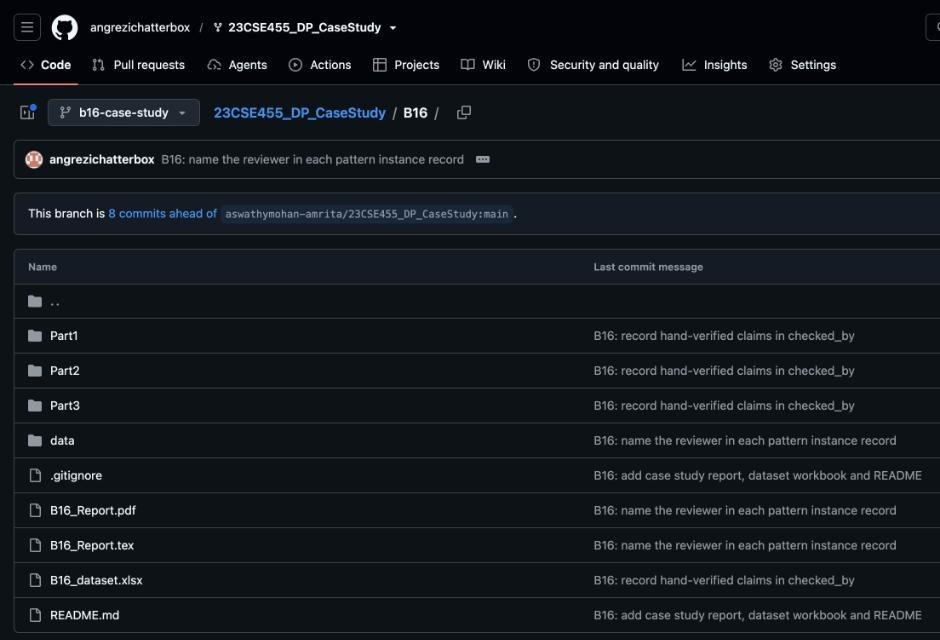
\includegraphics[width=\linewidth]{screenshots/1_B16.jpg}\caption{GitHub: \texttt{B16/}}\end{figure}
\begin{figure}[H]\centering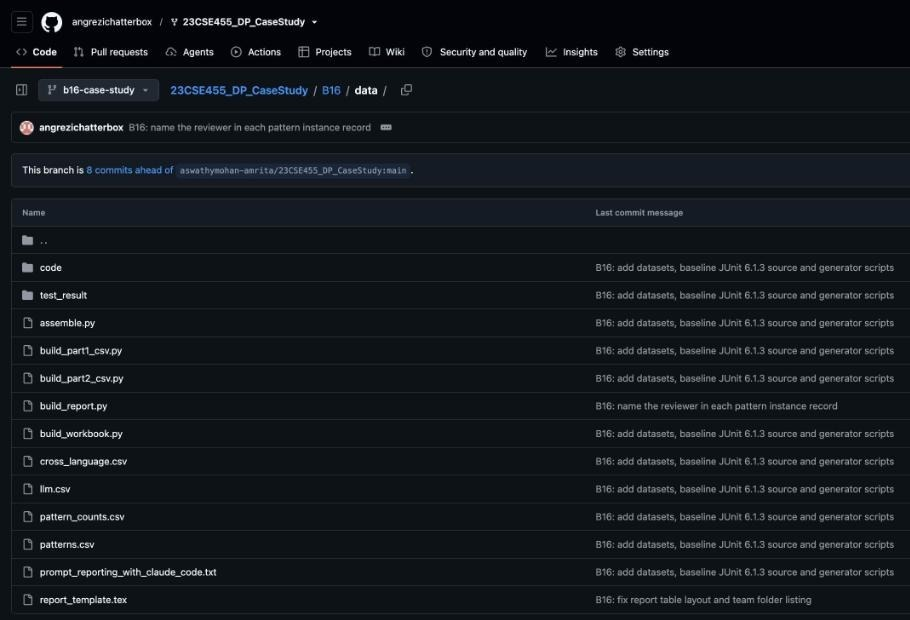
\includegraphics[width=\linewidth]{screenshots/2_data.jpg}\caption{GitHub: \texttt{B16/data/}}\end{figure}
\begin{figure}[H]\centering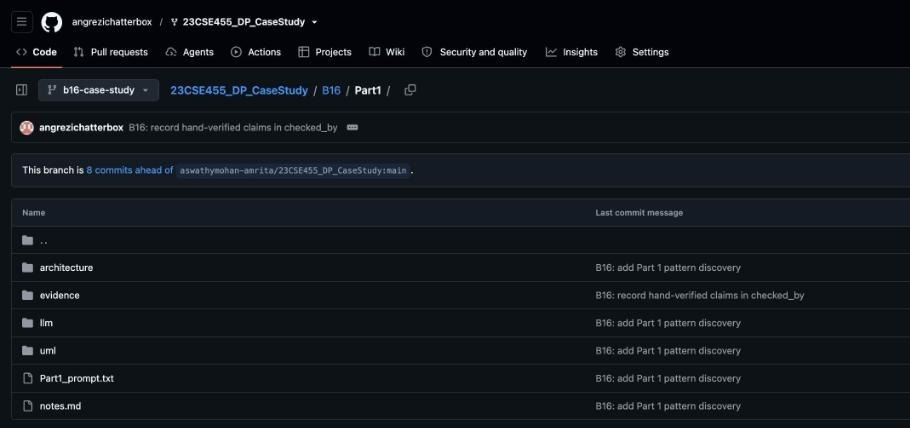
\includegraphics[width=\linewidth]{screenshots/3_Part1.jpg}\caption{GitHub: \texttt{B16/Part1/}}\end{figure}
\begin{figure}[H]\centering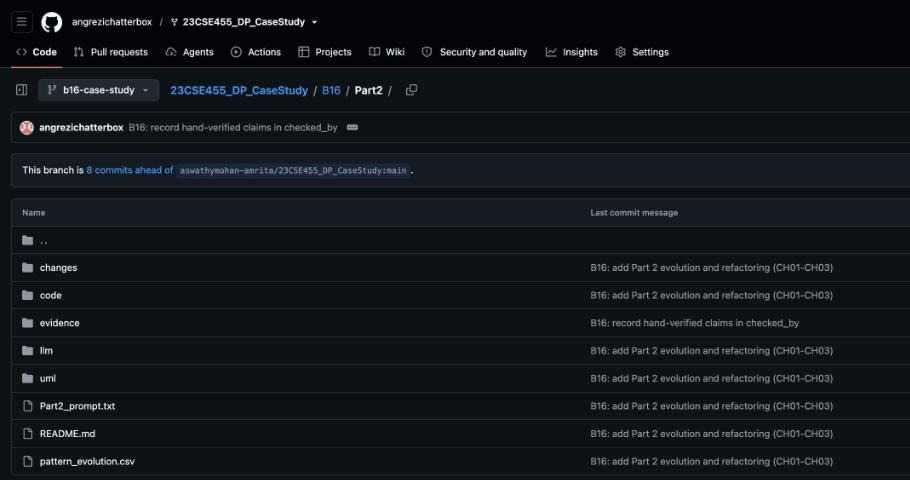
\includegraphics[width=\linewidth]{screenshots/4_Part2.jpg}\caption{GitHub: \texttt{B16/Part2/}}\end{figure}
\begin{figure}[H]\centering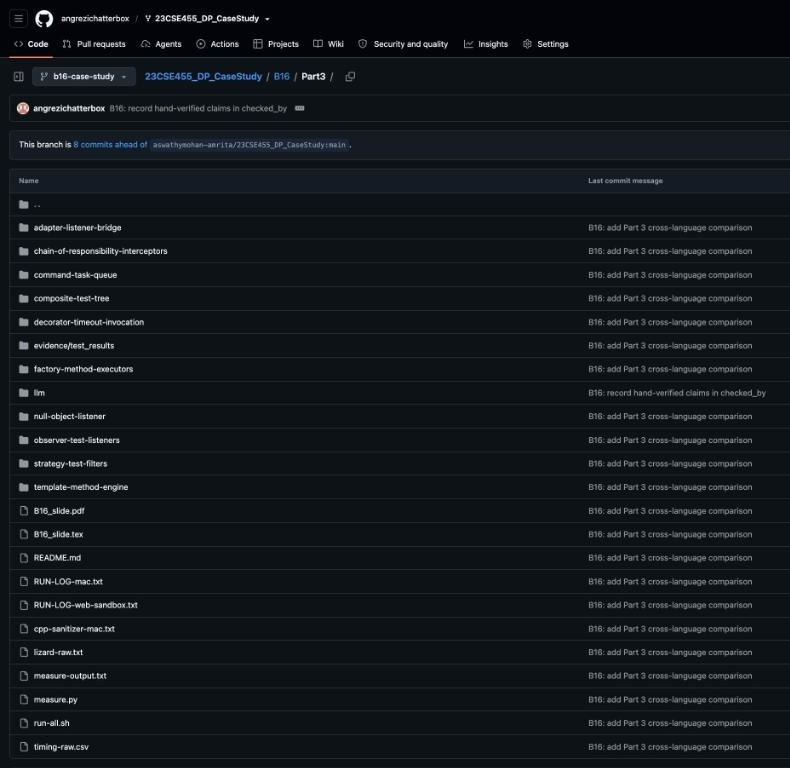
\includegraphics[width=\linewidth]{screenshots/5_Part3.jpg}\caption{GitHub: \texttt{B16/Part3/}}\end{figure}

\appendix
\section{UML diagrams changed in Part 2}\label{app:uml}
The diagrams that changed in Part~2 (\path{Part2/uml/}; new participants in green). Baseline diagrams for all 35 instances are not repeated here: they are in \path{Part1/uml/} (PlantUML sources and PNGs; 98 of 98 implements/extends arrows checked against the code), and each instance record above gives its path.

\begin{figure}[H]\centering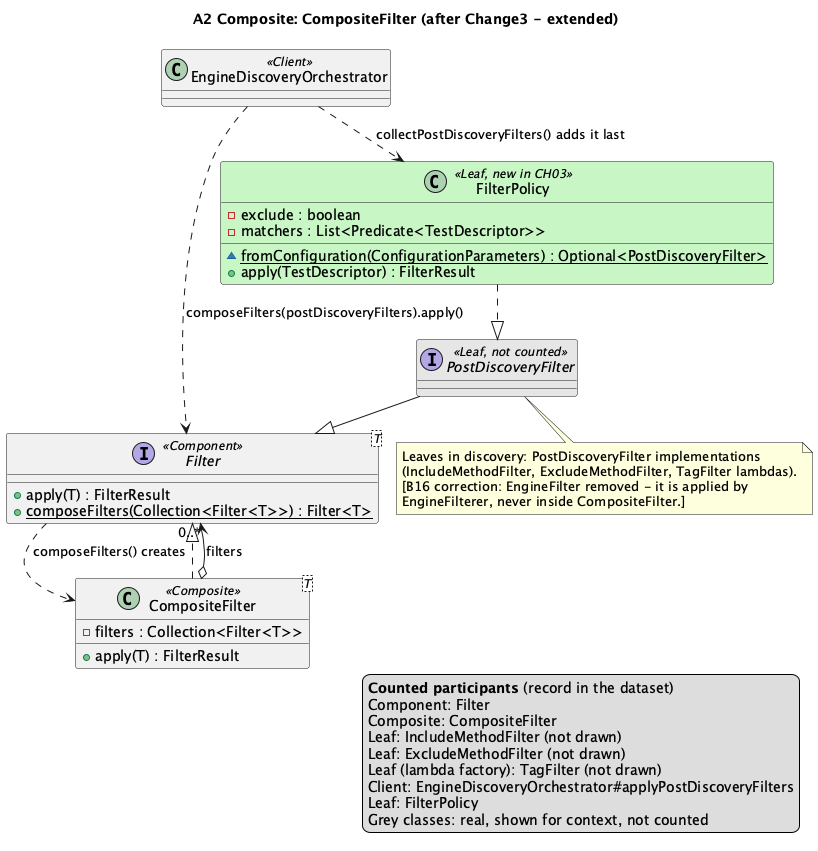
\includegraphics[width=0.95\linewidth,height=0.42\textheight,keepaspectratio]{Part2/uml/png/A2.png}\caption{A2 after Change3 (extended)}\end{figure}
\begin{figure}[H]\centering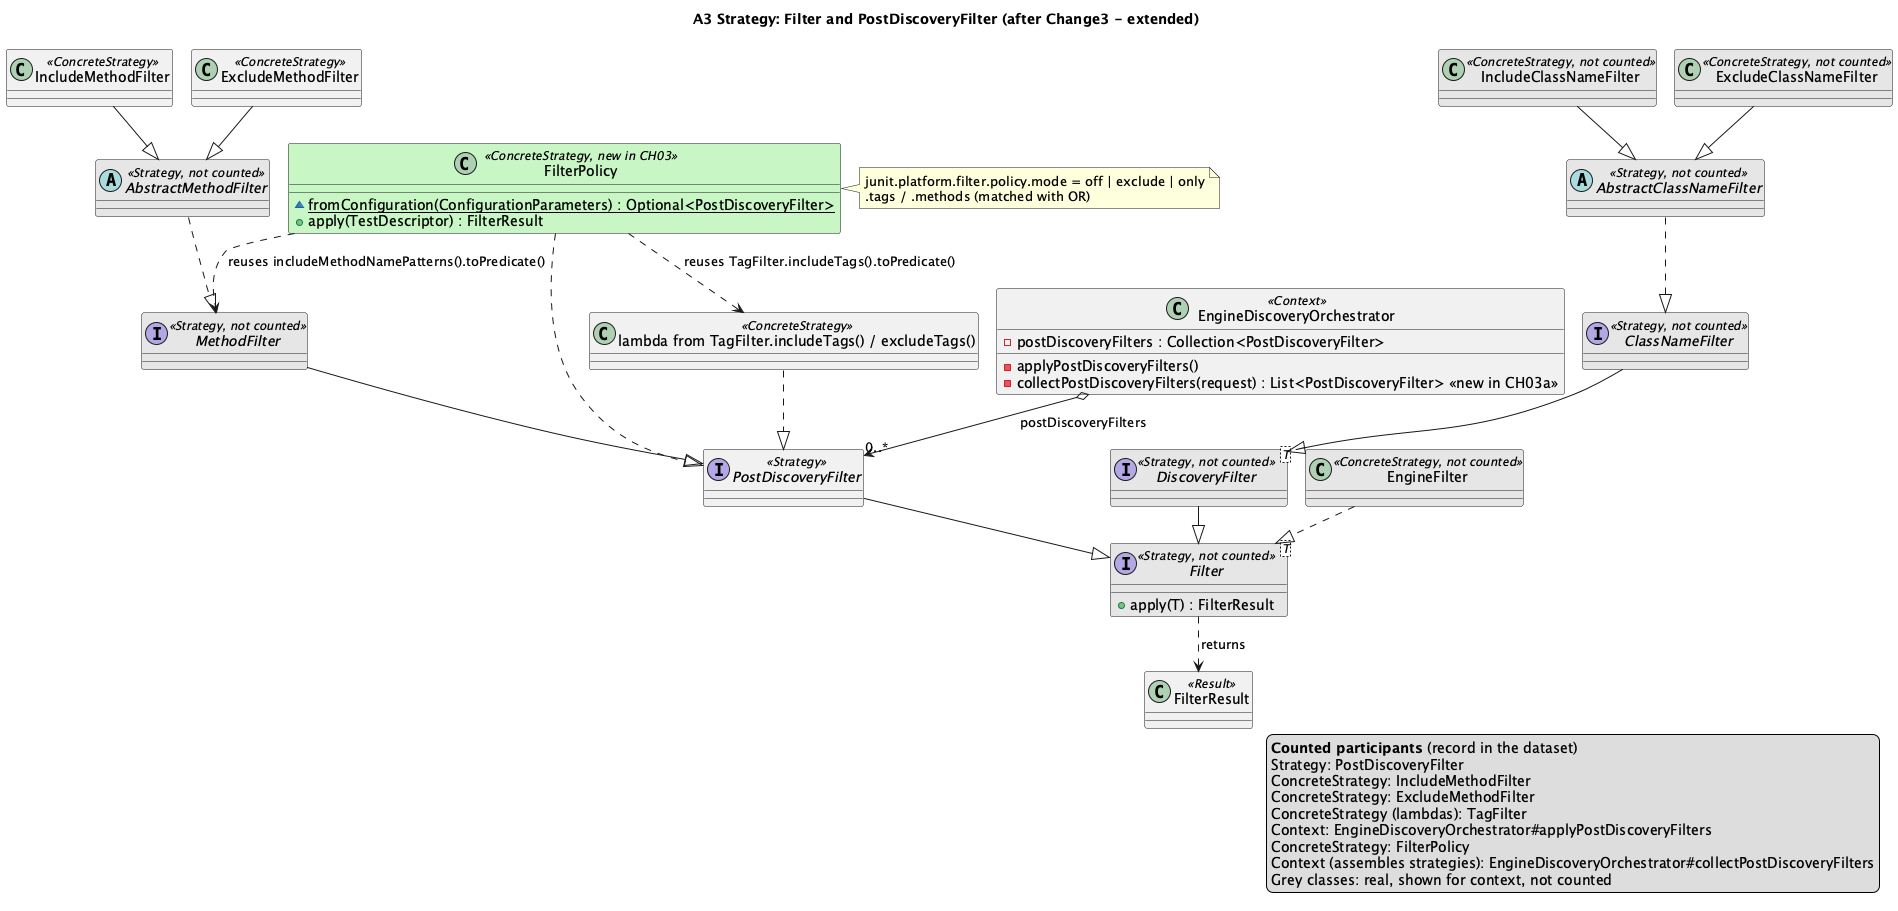
\includegraphics[width=0.95\linewidth,height=0.42\textheight,keepaspectratio]{Part2/uml/png/A3.png}\caption{A3 after Change3 (extended)}\end{figure}
\begin{figure}[H]\centering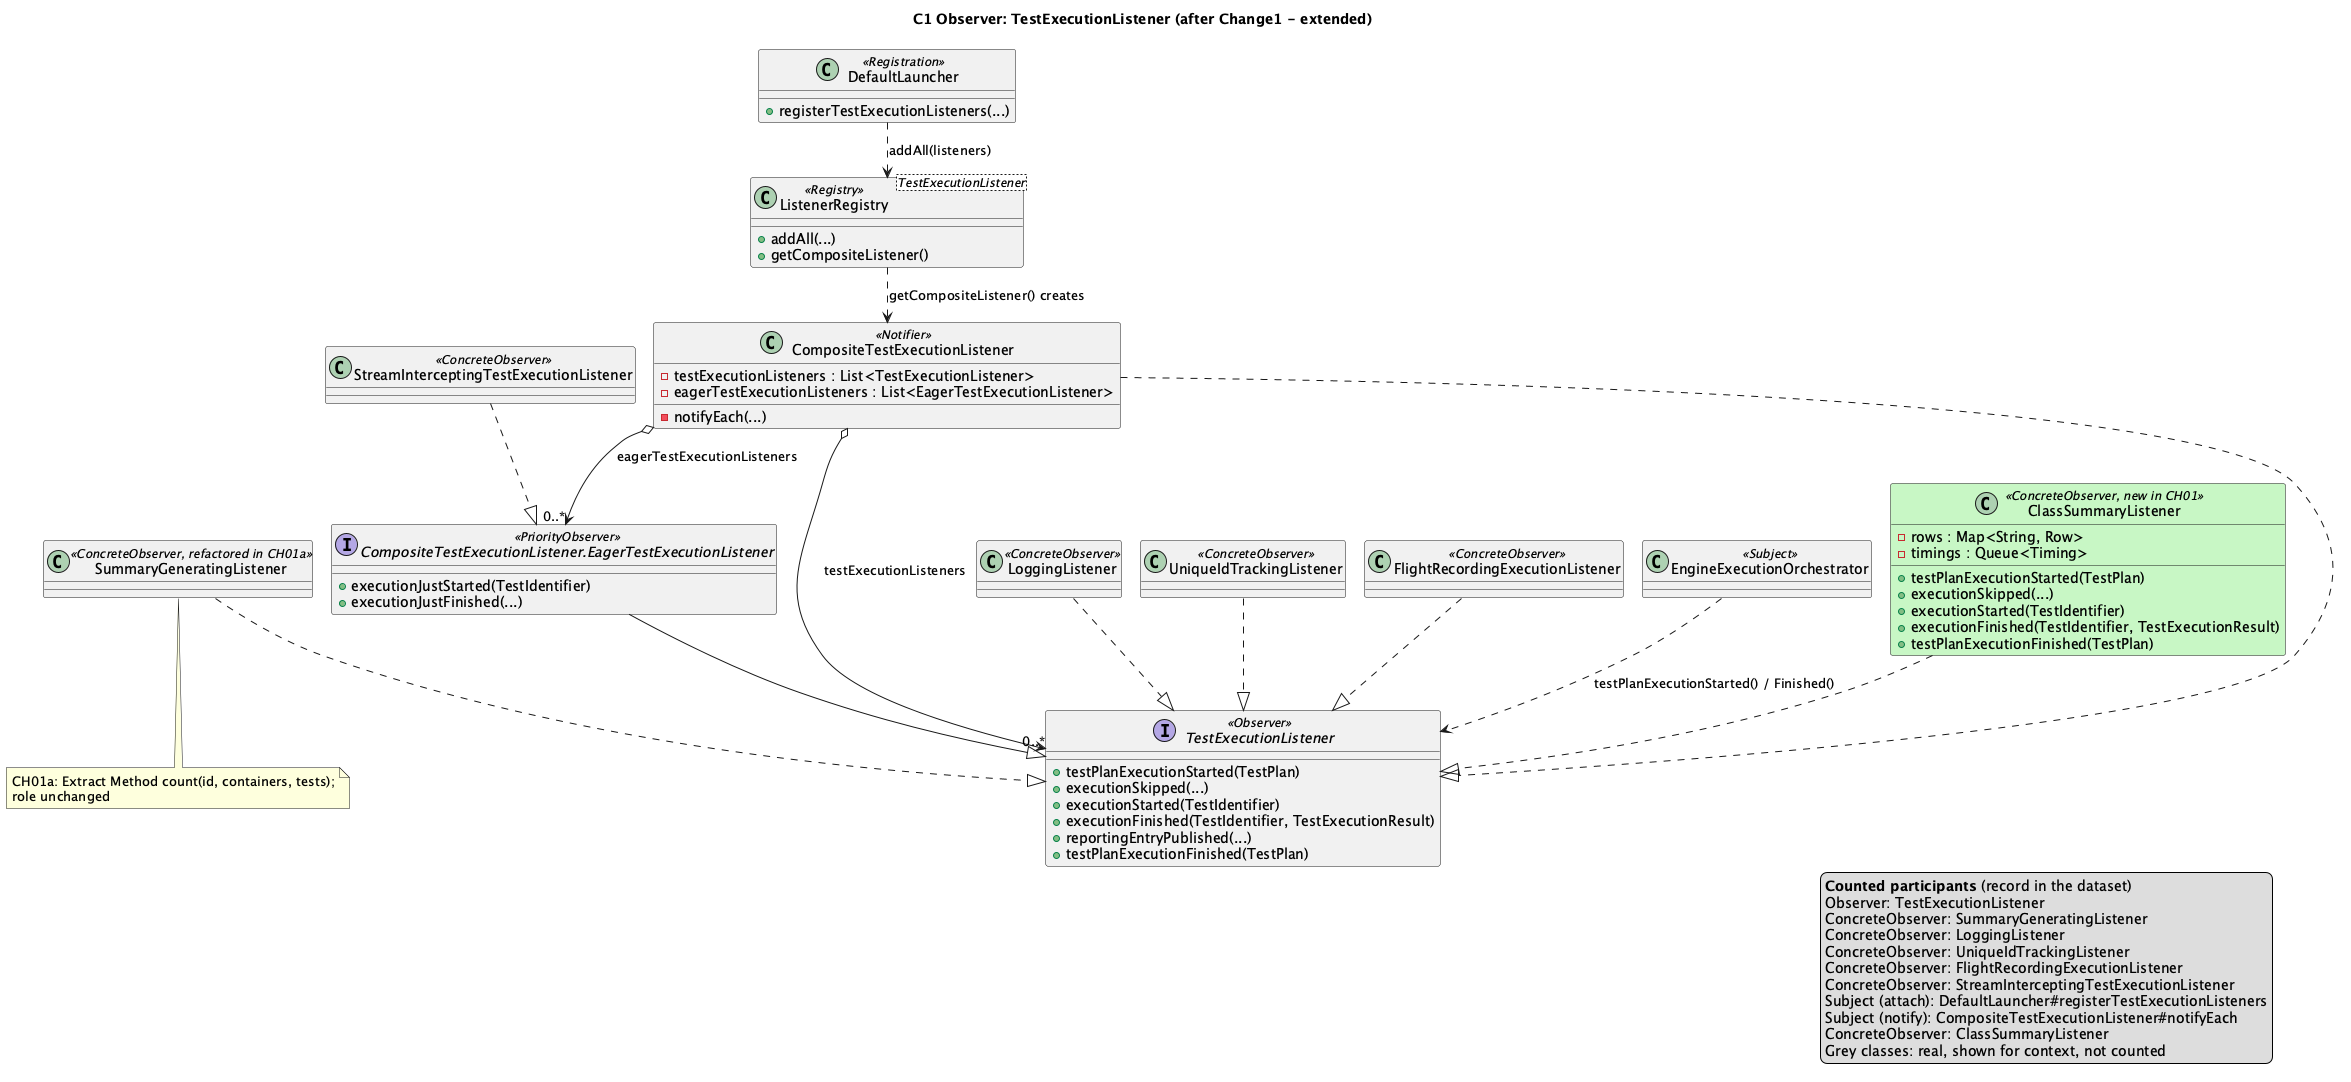
\includegraphics[width=0.95\linewidth,height=0.42\textheight,keepaspectratio]{Part2/uml/png/C1.png}\caption{C1 after Change1 (extended)}\end{figure}
\begin{figure}[H]\centering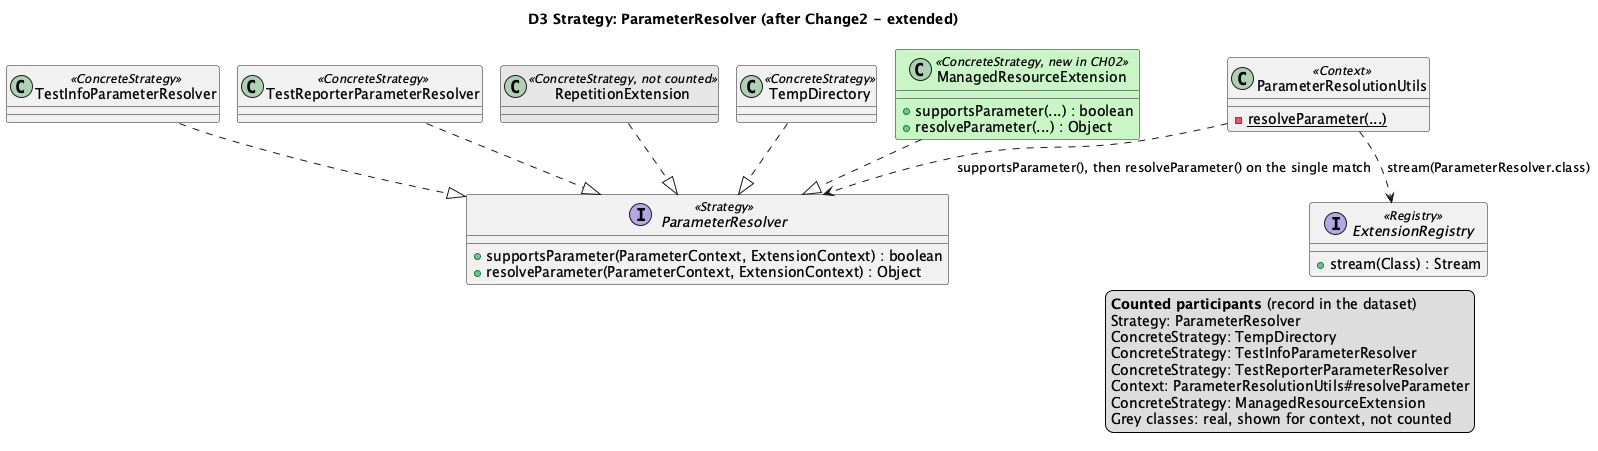
\includegraphics[width=0.95\linewidth,height=0.42\textheight,keepaspectratio]{Part2/uml/png/D3.png}\caption{D3 after Change2 (extended)}\end{figure}
\begin{figure}[H]\centering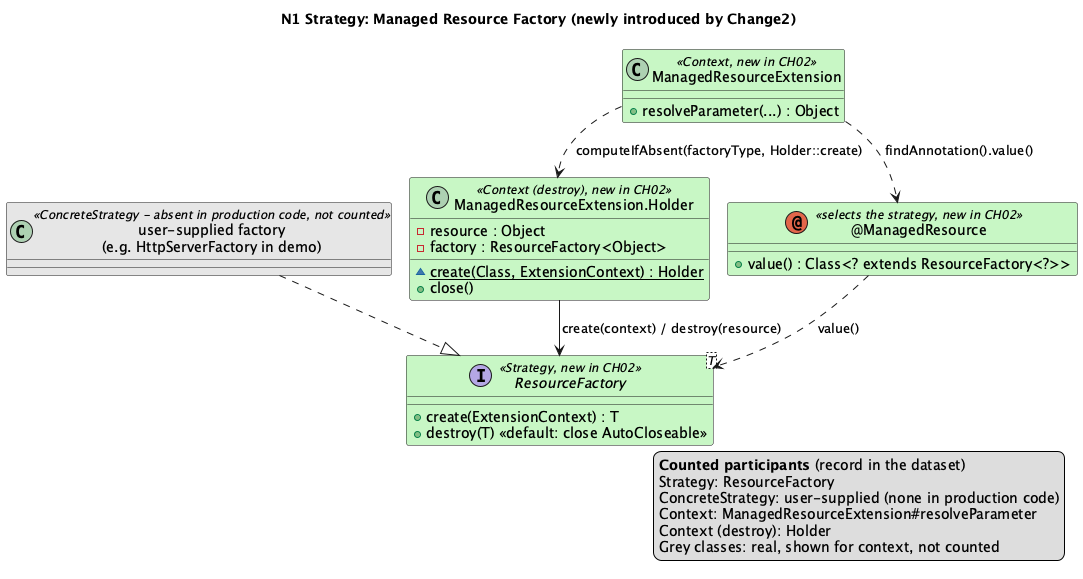
\includegraphics[width=0.95\linewidth,height=0.42\textheight,keepaspectratio]{Part2/uml/png/N1.png}\caption{N1 Managed Resource Factory (Strategy, newly introduced by Change2)}\end{figure}
\begin{figure}[H]\centering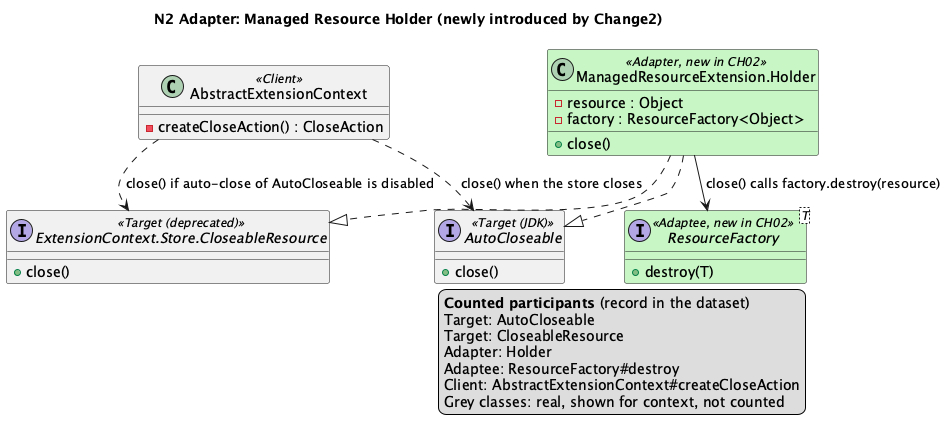
\includegraphics[width=0.95\linewidth,height=0.42\textheight,keepaspectratio]{Part2/uml/png/N2.png}\caption{N2 Managed Resource Holder (Adapter, newly introduced by Change2)}\end{figure}

\end{document}
